%% DKAP Paper --- PeerJ Computer Science submission
%% Converted from the canonical manuscript (paper/submission/bundle/main.tex).
%%
%% Submissions for peer review must enable line-numbering via the lineno
%% class option, per PeerJ author guidelines.
\documentclass[fleqn,10pt,lineno]{wlpeerj}

\usepackage[T1]{fontenc}
\usepackage{amssymb,amsfonts}
\usepackage{textcomp}
\usepackage{multirow}
\usepackage{array}
\usepackage{tabularx}
\usepackage{float}
\usepackage{url}
\usepackage[hidelinks]{hyperref}
\usepackage{bm}

% Table column types (used throughout the manuscript's tables)
\newcolumntype{L}[1]{>{\raggedright\arraybackslash}p{#1}}
\newcolumntype{C}[1]{>{\centering\arraybackslash}p{#1}}
\newcolumntype{R}[1]{>{\raggedleft\arraybackslash}p{#1}}

\title{Completeness over Structuring: A Controlled Text-to-SQL Ablation and Source-Code Analysis of Twenty-Nine AI Systems}

\author[1]{Dooil Kwak}
\affil[1]{Department of AI Techno Convergence, Graduate School, Soongsil University, Seoul, Republic of Korea}
\corrauthor[1]{Dooil Kwak}{babel.ai.dub@gmail.com}

% NOTE: wlpeerj.cls deliberately removed the \keywords{} macro in v1.2
% ("LLT 18 Aug 2016: no more keywords") -- PeerJ collects keywords as
% online-submission metadata rather than typesetting them in the PDF, so
% no \keywords{} call is made here. See the conversion report for detail.

\begin{abstract}
\textbf{Background.} Domain-specific AI systems increasingly inject structured domain knowledge---schemas, glossaries, ontologies, rule sets---into retrieval pipelines, but whether the structuring of that knowledge improves accuracy, or whether the completeness of the underlying information is what actually matters, is rarely tested in isolation. This study separates the two effects at two scopes: a descriptive, source-code-level analysis of real-world AI systems, and a controlled Text-to-SQL ablation.

\textbf{Methods.} We mined the architecture of twenty-nine real-world AI systems (thirteen industrial, sixteen open-source) spanning sixteen paradigms, identifying a recurring five-layer pattern---the Domain Knowledge Adaptation Pattern (DKAP)---defined by a knowledge-structuring layer (L2) that compiles domain knowledge offline into static artifacts consumed by a downstream retrieval and routing layer (L3). To isolate the effect of structuring from the effect of information quantity, we ran a controlled ablation on Text-to-SQL across three domains, six independent large language model (LLM) families, and ten seeds (approximately 9,000 runs), using four conditions---B1 (vanilla), B1\_DDL (schema-only diagnostic), B2 (flat-chunk retrieval), and DKAP (full)---plus an information-matched control (B2$'$) that supplies the identical domain knowledge as DKAP but as unstructured prose rather than structured artifacts.

\textbf{Results.} Information completeness is the primary, robust driver of accuracy: providing complete domain knowledge yields $+$26.0 percentage points (pp) in finance, replicating to a $+$17.5pp mean across six independent model families, positive for every family. Structuring that same information adds comparatively little: on the primary model it yields $+$5.3--7.7pp on easy/medium queries, but this does not generalize---across six model families the mean structuring gain is $+$0.7pp, with a 95\% confidence interval that includes zero. This null result is conservatively biased against DKAP, since the unstructured prose control incidentally carries elaborative reasoning cues that the structured artifacts lack. The combined benefit of supplying domain knowledge (completeness plus structure) scales with domain complexity, as characterized by a lightweight descriptive rubric, the Domain Knowledge Score (DKS): largest in the highest-complexity domain and absent in the lowest-complexity one.

\textbf{Conclusions.} For practitioners building domain-specific AI systems, the actionable implication is to secure complete domain knowledge before investing effort in how that knowledge is formatted---completeness, not structuring, is what reliably moves accuracy across model families. Controlled causal claims in this study are confined to Text-to-SQL; the cross-paradigm evidence for the five-layer pattern is architectural and descriptive, not experimental, and is offered to motivate future ablations in non-LLM paradigms.
\end{abstract}

\begin{document}

\raggedbottom
\maketitle
\thispagestyle{empty}
\section{Introduction}

Between 2024 and 2025, the author directly developed over 40 AI systems for industrial clients across heterogeneous domains, including finance, healthcare, public infrastructure, automotive manufacturing, shipbuilding process optimization, and entertainment. These systems ranged from early proof-of-concept deployments to full production rollouts; thirteen representative systems across seven industries were selected for the present analysis. Each domain imposed fundamentally different constraints: regulatory environments (HIPAA-equivalent for healthcare, K-ISMS for finance), data formats (OMOP CDM, the Observational Medical Outcomes Partnership Common Data Model, for medical, P6 scheduling for shipbuilding, engineering drawings for automotive), ontology systems (ICD/SNOMED CT for diseases, WBS for project management, BOM hierarchies for manufacturing), and security requirements (personally identifiable information [PII] masking for finance, IRB compliance for healthcare, classified document handling for public agencies).

Despite these radical differences, a recurring observation emerged: similar architectural decisions appeared across projects. The same fundamental questions---where to inject domain knowledge, how to structure retrieval, when to apply security filtering---were answered with structurally similar solutions across domains. In particular, one structural dependency recurred consistently: \textit{a layer that produces static domain artifacts (glossaries, schemas, ontologies) whose output determines the behavior of a downstream retrieval/routing layer}. This was not simply layered design; it was a specific producer--consumer interface between domain knowledge preparation and domain-conditioned execution. This empirical intuition motivated a systematic investigation.

Yet how much this structuring actually \textit{matters}---and whether its value comes from the structure itself or merely from the additional information it carries---has not been measured under controlled conditions. Existing domain adaptation research treats domain knowledge largely as a given input (a schema placed in the prompt, a corpus to retrieve from) and optimizes models or retrieval around it~\citep{finsql,ehrsql,korquad}; it has not isolated the effect of \textit{structuring} domain knowledge from the effect of simply providing \textit{more} of it. We position the present study to fill precisely this gap; the stream-specific gaps---in Text-to-SQL, RAG, compound AI systems, and model-level domain adaptation---are detailed in Section~\ref{sec:related}.

Because the five layers of this pattern---developed in Section~3 as the Domain Knowledge Adaptation Pattern (DKAP)---are referenced by their short labels (L1--L5) throughout the paper before they are formally defined, Table~\ref{tab:layers_glance} summarizes them up front for orientation. The experiments center on Layer~2 (knowledge structuring) and its hand-off to Layer~3 (retrieval); the full architecture is presented in Section~3.

\begin{table}[H]
\centering
\caption{The five DKAP layers at a glance (orientation only). The full architecture is developed in Section~3. LLM = large language model; RL = reinforcement learning; VLM = vision-language model; ML = machine learning.}
\label{tab:layers_glance}
\footnotesize
\begin{tabularx}{\columnwidth}{@{}lX@{}}
\toprule
\textbf{Layer} & \textbf{Role} \\
\midrule
L1 Input Processing & Normalize and route the incoming request \\
L2 Knowledge Structuring & Compile domain knowledge offline into \textit{static} artifacts (glossaries, ontologies, schemas, rule sets) \\
L3 Retrieval / Routing & Consume the L2 artifacts at query time for domain-conditioned retrieval \\
L4 AI Inference & Engine-agnostic core (LLM, RL, VLM, or ML) \\
L5 Validation & Verify and audit the output \\
\bottomrule
\end{tabularx}
\end{table}

This paper therefore addresses three research questions:

\noindent\textbf{RQ1 (effect vs.\ information quantity):} When domain knowledge is structured into explicit artifacts (L2), is the resulting performance benefit \textit{separable} from the benefit of simply providing more information?

\noindent\textbf{RQ2 (boundary conditions):} Does the L2 benefit \textit{appear to vary} with the domain's knowledge complexity?

\noindent\textbf{RQ3 (paradigm-generality):} Does the five-layer organization, and the L2$\rightarrow$L3 producer--consumer dependency, appear regardless of the underlying AI engine---large language model (LLM), reinforcement learning (RL), or machine learning (ML)?

Our contributions follow directly from these questions. The single core argument is that domain knowledge structuring is a distinct, separable architectural concern whose performance contribution can be measured---and, when measured carefully, turns out to be more nuanced than ``more structure is always better.''

\noindent\textbf{(C1) Controlled measurement of the structuring effect.} Through ablation experiments on three Text-to-SQL domains, including an information-matched control condition (B2$'$) that supplies the same domain knowledge as the full system in unstructured prose, we isolate the effect of \textit{structuring} from the effect of \textit{information quantity}. We find that information completeness is the primary driver of accuracy ($+$26.0pp over flat-chunk retrieval in finance), and a six-model cross-validation on the finance ablation shows this completeness gain replicates robustly ($+$17.5pp on average, positive for all six independent model families; see Table~\ref{tab:crossmodel} and Fig.~\ref{fig:teaser}), whereas the structuring gain over information-matched prose does not generalize (mean $+$0.7pp, 95\% CI includes zero; $+$5.3--7.7pp on the primary model only). This calibrated, cross-model decomposition---rather than an inflated end-to-end gain---is our primary contribution (C2 and C3 below are supporting apparatus). Because practitioners routinely invest in structuring domain knowledge before securing its completeness, a calibrated null on structuring is itself actionable: it reorders the engineering priorities toward completeness first. The descriptive apparatus (C2, C3) is not in tension with this null but answers its natural follow-up---where the combined L2 benefit is worth securing at all: DKS is the instrument that separates the high-complexity regime where it pays off from the low-complexity regime where even completeness adds nothing semantic (Section~\ref{sec:cross_domain_summary}).

\noindent\textbf{(C2) A descriptive framework grounding the experiment.} To organize and motivate this measurement, we characterize a recurring five-layer organization (DKAP) through source-code-level analysis of twenty-nine AI systems spanning sixteen paradigms (including five non-LLM systems), in which a dedicated layer (L2) produces static domain artifacts consumed downstream (L3). We use DKAP as a descriptive lens, not a claimed architectural invention; the individual layers are familiar engineering concerns. The L2$\rightarrow$L3 producer--consumer dependency recurs across LLM-, RL-, and ML-based systems (RQ3), suggesting---without proving---that it is not an LLM-specific convention.

\noindent\textbf{(C3) A lightweight descriptive instrument.} To \textit{describe}---not evaluate---domain knowledge complexity, we provide a scoring rubric---the Domain Knowledge Score (DKS), the dominant subscale of our combined DKS and Retrieval Sophistication Score (RSS) rubric. We report its reliability---cross-family agreement across seven independent LLM judge lineages (Krippendorff's $\alpha = 0.718$; mean pairwise Spearman $\rho = 0.782$) and author--ensemble agreement ($\rho = 0.786$, $p = 0.002$)---and its positive association with pipeline depth (external-only Pearson $r = 0.857$, $p < 0.001$) as supporting analyses, not as the paper's primary evidence. We are explicit that this reliability claim is limited to rank-order agreement, not absolute scores: families differ in generosity, and the interval-scale bootstrap CI is wide (Section~\ref{sec:limitations}). The rubric is a quasi-ordinal complexity \textit{descriptor}, and independent human validation remains future work.

For practitioners building an AI system in a new domain, the practical implication is concrete: secure complete domain knowledge \textit{before} selecting or tuning a model---its payoff grows with domain complexity---while explicit structuring chiefly buys added precision on easy-to-medium schema mapping.


%% ============================================================
%%  SECTION 2: RELATED WORK
%% ============================================================
\section{Related Work}
\label{sec:related}

We position this work at the intersection of three research streams, each of which addresses a fragment of the problem but none of which captures the full picture of cross-domain architectural patterns.

\subsection{Text-to-SQL and Domain-Specific NL Interfaces}

The Text-to-SQL community has produced increasingly sophisticated benchmarks and models: Spider~\citep{spider} established cross-database evaluation, BIRD~\citep{bird} introduced large-scale real-world databases, FinSQL~\citep{finsql} specialized for financial schemas, and EHRSQL~\citep{ehrsql} targeted clinical environments. These works demonstrate that domain-specific schema understanding dramatically improves natural language query accuracy. However, they treat domain knowledge as a given input (schema provided in the prompt) rather than investigating how that knowledge should be structured, organized, and injected into the system pipeline.

A complementary line of work examines knowledge representation \textit{within} the prompting pipeline: \citet{chang2023prompt} systematically ablate schema serialization formats (table--column lists vs.\ data-definition-language (DDL) statements, database content representations) under controlled conditions; \citet{dailsql} (DAIL-SQL) comprehensively evaluate how question and schema knowledge should be encoded in the prompt; and \citet{maamari2024death} show that for recent reasoning-capable LLMs, supplying the complete schema can dominate explicit schema-linking---a coverage-over-structuring finding directionally consistent with ours; we extend it from a within-prompt, single-model observation to a controlled, system-architecture-level result tested across six independent model families (Section~\ref{sec:crossmodel}). These studies vary knowledge representation within a single prompt; our work asks the analogous question at the system-architecture level. L2 of DKAP formalizes the domain knowledge structuring process that Text-to-SQL systems implicitly assume.

\subsection{Retrieval-Augmented Generation (RAG) and Structuring}

Since \citet{lewis2020rag} established that external knowledge retrieval enhances LLM performance, RAG has become the dominant paradigm for knowledge-grounded generation~\citep{gao2024rag,fan2024survey}.

Subsequent work has explored advanced retrieval strategies: multi-hop reasoning~\citep{chen2019multihop}, adaptive retrieval timing~\citep{selfrag}, retrieval-augmented fine-tuning~\citep{radit}, and composable LLM application frameworks~\citep{chase2025langchain}. These studies comprehensively answer ``what to retrieve'' but leave unexplored ``how to structure domain knowledge so that retrieval becomes effective.''

Most recently, \citet{jiang2025ras} surveyed Retrieval And Structuring (RAS) Augmented Generation, which extends RAG by incorporating text structuring techniques---taxonomy construction, hierarchical classification, and information extraction---that transform unstructured text into organized representations before or during LLM inference.

RAS represents the closest related work to DKAP's L2 layer, as both recognize that \textit{structuring} domain knowledge is a distinct concern from retrieval. However, DKAP differs from RAS in three respects: \textbf{scope}---RAS structures text within the LLM prompting pipeline, whereas DKAP's L2 is a system-level layer applying regardless of AI engine (LLMs, RL agents, vision-language models (VLMs), ML ensembles); \textbf{granularity}---RAS operates at the text/document level (e.g., entity--relation triples), whereas L2 encompasses richer artifacts (domain ontologies, cross-standard mappings such as ICD$\leftrightarrow$SNOMED, SQL schemas, regulatory encodings, multi-language term tables) that often predate any LLM; and \textbf{methodology}---RAS is a taxonomy of techniques, whereas DKAP is an empirically observed pattern inductively derived from twenty-nine systems with a quantitative complexity metric (DKS).

In practice, we observe that RAG performance degrades significantly when the relevant domain knowledge is not prepared upstream (e.g., unstructured medical documents without OMOP CDM alignment, financial data without PII taxonomy). DKAP makes this dependency explicit by separating the knowledge-structuring layer (L2) from retrieval (L3), positing that effective RAG requires a dedicated upstream knowledge layer. RAS provides evidence that the RAG community is independently converging on a similar insight, which we interpret as corroborating our empirical observation. Recent controlled comparisons of graph-structured versus flat retrieval on identical corpora~\citep{xiang2026graphragbench} likewise find that the benefit of structuring is conditional on task regime rather than uniform---consistent with the boundary conditions we report in Section~\ref{sec:cross_domain_summary}.

\subsection{Compound AI Systems and Agentic Architectures}

A parallel line of work has shifted attention from individual models to multi-component AI systems. \citet{zaharia2024compound} introduced the \textit{compound AI system} paradigm, arguing that state-of-the-art AI applications increasingly consist of multiple interacting components---retrievers, verifiers, orchestrators---rather than a single model. Their analysis identifies knowledge management as a first-class architectural concern, but does not formalize how domain-specific knowledge should be structured within these components.

Concurrently, orchestration frameworks such as LangGraph~\citep{chase2025langchain} and CrewAI~\citep{crewai} have operationalized multi-step AI pipelines; our analysis shows that these frameworks score low on DKS (LangGraph/LangChain: generic RAG infrastructure with no built-in domain knowledge; CrewAI: DKS$=$15) precisely because they defer domain knowledge structuring to user configuration.

The compound AI perspective reinforces DKAP's positioning: while compound AI systems describe \textit{what components exist}, DKAP characterizes \textit{how domain knowledge should flow between them}---specifically, that L2 (structured domain artifacts) must precede L3 (domain-conditioned retrieval) as a producer--consumer relationship. GraphRAG~\citep{graphrag} provides a recent concrete example: its two-phase architecture (offline graph construction + online retrieval) maps directly to DKAP's L2$\to$L3 interface, with the knowledge graph serving as the L2 static artifact consumed by query-time retrieval.

\subsection{Domain Adaptation in Machine Learning}

Domain adaptation research spans fine-tuning~\citep{howard2018ulmfit}, prompt tuning~\citep{lester2021prompt}, adapter layers~\citep{houlsby2019adapter}, source-free domain adaptation~\citep{liang2020sourcefree}, and agentic memory mechanisms~\citep{zhang2024agentic}. These approaches operate at the model parameter level---adapting learned representations to new domains through gradient-based optimization.

While effective for within-model transfer, they do not address the system architecture level: how input normalization, knowledge structuring, retrieval routing, inference fallback, and output validation should be organized across domains. DKAP occupies a complementary position: it is a system-level domain adaptation pattern that can be applied regardless of whether the underlying model uses fine-tuning, prompt engineering, or reinforcement learning. Fig.~\ref{fig:positioning} illustrates this positioning.

Fig.~\ref{fig:positioning} organizes existing approaches along two axes: optimization focus (model-centric vs.\ architecture-centric) and scope (single-domain vs.\ cross-domain). Model-centric single-domain work (FinSQL~\citep{finsql}, EHRSQL~\citep{ehrsql}, Spider/BIRD~\citep{spider,bird}) optimizes model parameters for one domain. Model-centric cross-domain work (domain adaptation~\citep{wang2018domain}, fine-tuning/LoRA) transfers model weights across domains. Architecture-centric single-domain work (Self-RAG~\citep{selfrag}, RA-DIT~\citep{radit}) designs retrieval pipelines for specific tasks. DKAP uniquely occupies the architecture-centric, cross-domain quadrant: it is a domain-transferable architectural pattern inductively derived from real industrial codebases, agnostic to both AI engine and domain.

\begin{figure}[H]
\centering
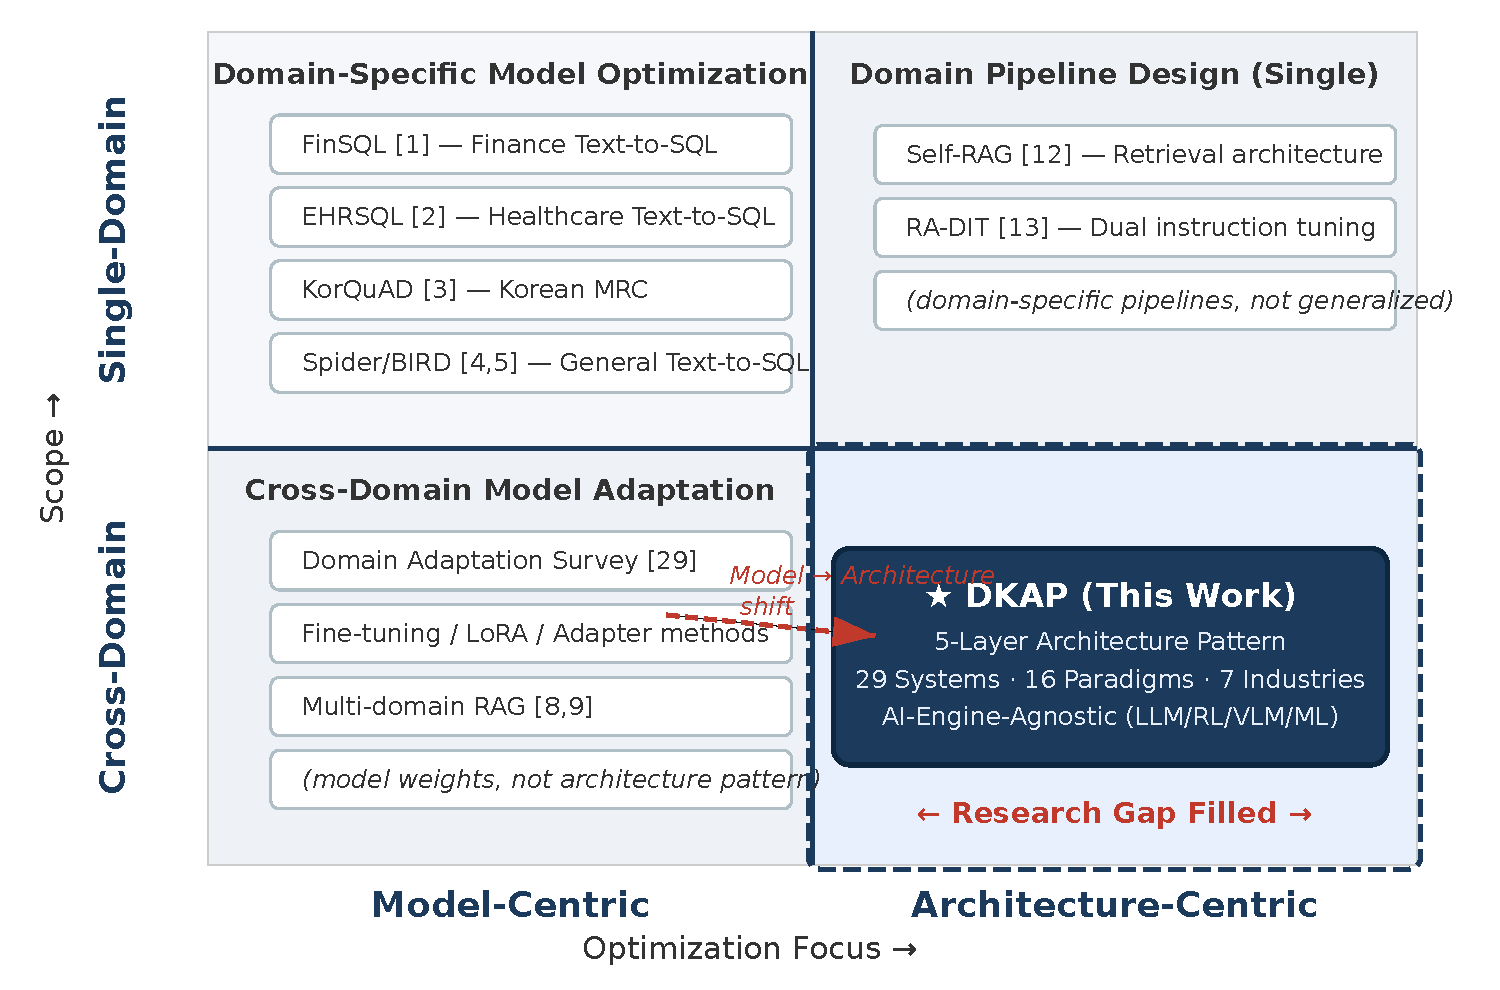
\includegraphics[width=\textwidth]{Fig1_DKAP_Positioning_Matrix}
\caption{Positioning of DKAP relative to existing approaches, organized by optimization focus (model-centric vs.\ architecture-centric) and scope (single- vs.\ cross-domain). Prior work clusters in the model-centric and single-domain pipeline quadrants; DKAP occupies the architecture-centric, cross-domain quadrant that they leave open.}
\label{fig:positioning}
\end{figure}

\subsection{Empirical Studies of AI System Architecture}

Methodologically, this paper follows the empirical software engineering tradition of deriving patterns and taxonomies from many real systems. \citet{amershi2019se4ml} derived a nine-stage ML workflow and a maturity model from practitioner data inside one company; \citet{humbatova2020taxonomy} inductively built a fault taxonomy from mined artifacts with a multi-rater labeling protocol and validation survey; \citet{nahar2025product} mined open-source ML product repositories at the source-code level to characterize recurring architectural practices; and \citet{kreuzberger2023mlops} synthesized an end-to-end MLOps reference architecture from triangulated literature, tool, and interview evidence.

These studies establish the derive-then-validate template we adopt---explicit selection criteria, protocol-driven artifact analysis, reliability assessment---but address the ML development process, fault landscape, or operations infrastructure in general. \citet{sculley2015debt} influentially framed data dependencies as a primary, under-recognized source of architectural ``technical debt'' in ML systems, motivating the treatment of knowledge management as a first-class architectural concern; DKAP makes that concern explicit and measurable as the L2 layer.

None of these works isolates domain knowledge structuring as a measurable architectural concern, and none pairs the inductively derived pattern with a controlled ablation of the concern it identifies, which is the combination this paper contributes.

\subsection{Summary of Gaps}

Unlike model-centric domain adaptation approaches~\citep{wang2018domain,selfrag,radit} that optimize model parameters or retrieval mechanisms for specific tasks, DKAP addresses the complementary question of system-level architectural patterns inductively derived from real industrial codebases.

\textbf{What is specifically new.} The individual layers of DKAP (input processing, knowledge management, retrieval, inference, validation) are familiar engineering concerns, and we do not claim novelty for the layers themselves. Our specific contribution is methodological and empirical: using an information-matched control condition (B2$'$), we isolate the performance effect of \textit{structuring} domain knowledge from the effect of providing more information, and find that completeness is the primary driver while the structuring effect, once information is matched, is not distinguishable from zero across six independent model families.

This is distinct from prompt-level studies of schema representation---where \citet{maamari2024death} and \citet{zhang2026samecontent} vary how knowledge is serialized within a single model's prompt: we instead hold information fixed at the \textit{system-architecture} level (a dedicated L2 structuring layer versus equivalent prose) and test the effect across a six-family, multi-seed panel, turning a single-model, prompt-format observation into a cross-model, statistically bounded architectural result.

What no prior work establishes---and a single-model prompt study cannot yield---is the \textit{conjunction}: that the completeness-over-structuring decomposition (i)~survives the move from a within-prompt edit to a dedicated architectural layer, (ii)~holds across six independent model families rather than one, and (iii)~concerns exactly the L2 structuring layer we independently find recurring across twenty-nine real-world systems. Establishing all three together---not the direction of any one effect---is the novel result.

The five-layer DKAP decomposition is the descriptive framework that motivates and organizes this experiment; the positive association between L2 complexity and pipeline depth across independently developed systems is reported as \textit{supporting} evidence, not as the central claim. The contribution lies not in naming the layers, but in measuring---under controlled conditions---what structuring domain knowledge actually buys.

A natural question arises: how does DKAP differ from established software architecture patterns? We systematically compare DKAP with four canonical patterns~\citep{garlan1993intro,bass2021practice,newman2021microservices,richards2020fundamentals}:

\begin{itemize}[leftmargin=*,itemsep=2pt]
\item \textbf{N-tier Architecture} decomposes systems into horizontal layers (presentation, business logic, data). DKAP shares this layered principle but differs in that L2 produces \textit{static domain artifacts} (glossaries, ontologies, schemas) consumed by L3 at runtime---a producer--consumer relationship where the artifact format is domain-determined, not a uniform interface as in N-tier.

\item \textbf{Pipe-and-Filter} defines sequential processing stages with uniform data flow. DKAP's five layers superficially resemble a pipeline, but L2$\to$L3 is an asymmetric dependency: L2 artifacts are compiled offline and consumed at inference time, unlike Pipe-and-Filter where each stage transforms and forwards a uniform data stream.

\item \textbf{Microservices}~\citep{newman2021microservices} decompose systems into independently deployable services organized around business capabilities. While microservice AI systems exist (e.g., separate retrieval and inference services), microservices prescribe \textit{organizational} boundaries; DKAP prescribes \textit{knowledge-structural} boundaries. A microservice architecture might split L3 and L4 into separate services, but without DKAP's insight, L2 artifacts would be scattered across services rather than consolidated as a dedicated layer.

\item \textbf{Hexagonal Architecture} (Ports and Adapters)~\citep{richards2020fundamentals} isolates domain logic from external interfaces via adapter layers. DKAP's L1 (input normalization) and L5 (output validation) are analogous to adapters, but the core distinction is L2: Hexagonal Architecture assumes domain logic resides in application services; DKAP observes that in AI systems, domain knowledge must be \textit{externalized as structured artifacts} separate from the inference engine, because the AI engine (L4) is typically domain-agnostic.
\end{itemize}

In summary, DKAP is best understood as a \textit{domain-specific refinement} of layered architecture for AI systems, not a wholly novel architectural paradigm. Its specific contribution is identifying L2 (Domain Knowledge Structuring) as a distinct, measurable architectural concern---a layer that existing patterns do not anticipate because they predate the era of domain-agnostic AI engines that require explicit knowledge injection.

%% ============================================================
%%  SECTION 3: METHOD
%% ============================================================

%% ============================================================
%%  SECTION 3: MATERIALS \& METHODS
%% ============================================================
\section{Materials \& Methods}


\subsection{System Selection Criteria}

From 40+ industrial PoC systems developed between 2024--2025, we selected thirteen internal systems using stratified sampling along four dimensions: (1) domain diversity (seven distinct industries), (2) AI engine diversity (LLM, RL, vision-language model (VLM), ML ensemble), (3) data modality diversity (text, structured data, images, audio), and (4) pipeline complexity range (5--16 stages).

To mitigate single-source bias, we additionally analyzed sixteen external open-source systems. External systems were selected using the following inclusion criteria: (i) peer-reviewed publication or $\geq$1,000 GitHub stars as a quality threshold; (ii) publicly available source code sufficient for Architecture Mining Protocol application; (iii) one system per AI paradigm to maximize paradigm diversity (no two external systems share the same primary paradigm); (iv) at least four non-LLM systems to test engine-agnosticism.

We did \textit{not} exclude systems that might weaken the DKAP hypothesis; for instance, Pulse AI~\citep{pulseai} (DKS$=$14, 6 stages) and CrewAI (DKS$=$15, 7 stages) are included despite being minimal or framework systems with low domain structuring. We acknowledge that this selection process, while systematic, involves researcher judgment and cannot fully eliminate selection bias.

An inventory of considered-but-excluded systems and exclusion rationale, covering both the internal and external tracks, is provided in the Supplemental Material. Fig.~\ref{fig:funnel} summarizes the selection funnel for both tracks. For clarity on the subsets used later: of these sixteen external systems, thirteen are paradigm-matched to an internal system in the cross-validation of Section~\ref{sec:crossval} and three (Haystack~\citep{haystack}, AutoGPT~\citep{autogpt}, Rasa~\citep{rasa}) are unpaired; the cross-family rubric-reliability study (Section~\ref{sec:limitations}) scores the thirteen for which structured source-code evidence was available.

\begin{figure}[tp]
\centering
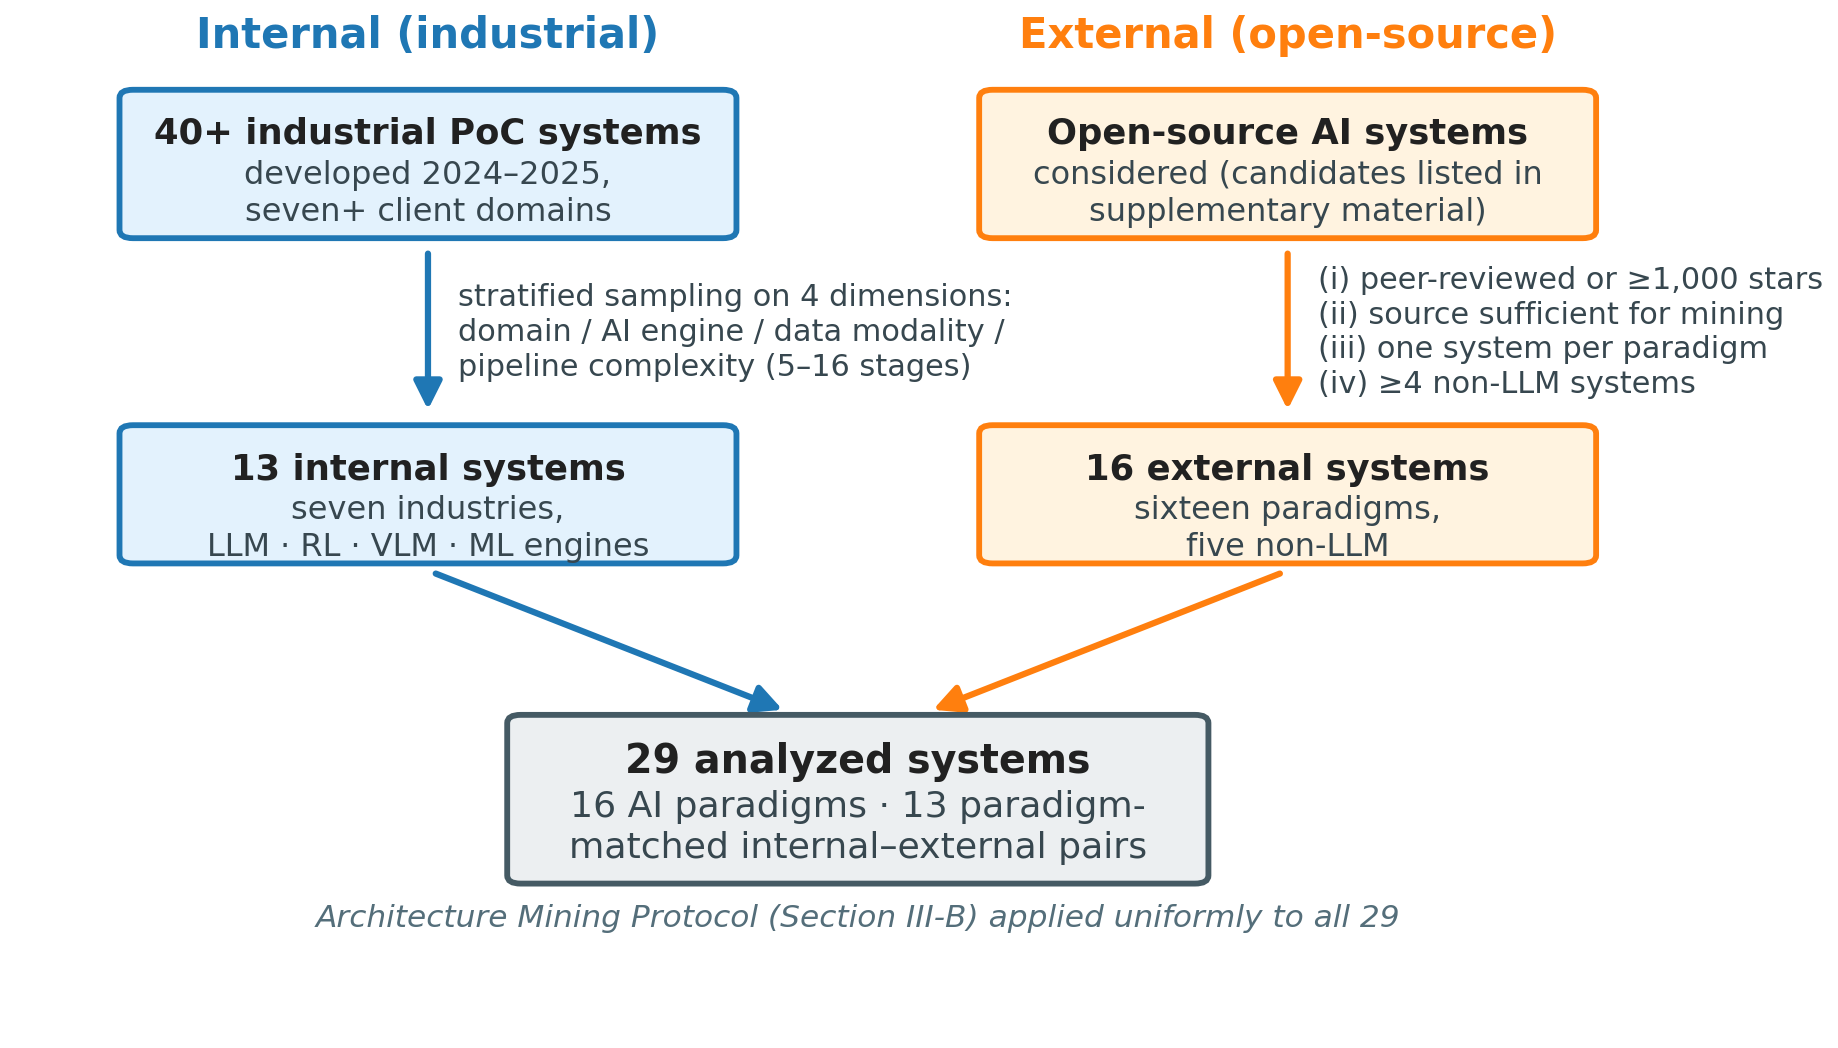
\includegraphics[width=\textwidth]{fig5_selection_funnel.png}
\caption{System selection funnel. Internal track: 40+ industrial PoC systems (2024--2025) reduced to thirteen by stratified sampling along four dimensions (domain, AI engine, data modality, pipeline complexity). External track: open-source candidates filtered by four inclusion criteria to sixteen systems spanning sixteen paradigms, including five non-LLM systems. The Architecture Mining Protocol (Section~3.2) is applied uniformly to all twenty-nine.}
\label{fig:funnel}
\end{figure}

\subsection{Architecture Mining Protocol}

To ensure systematic and reproducible analysis, we followed a four-step protocol:

\textit{Step 1 (Component Decomposition):} Each system's source code was decomposed into functional modules by analyzing Python/C\# package structures, API endpoint definitions, and service class hierarchies.

\textit{Step 2 (Data Flow Tracing):} For each system, we traced the complete data flow from user input entry point to final response output, documenting every intermediate processing stage.

\textit{Step 3 (Layer Assignment):} Each processing stage was assigned to one of five candidate layers based on its primary function: input normalization, knowledge structuring, retrieval/routing, AI inference, or output validation. The assignment criterion is: L2 produces structured domain artifacts (static representations); L3 consumes those artifacts at runtime to condition retrieval and routing (dynamic execution logic). Each stage receives exactly one primary-function assignment. Stage assignment is therefore distinct from layer \textit{presence}: a system can implement a layer's function at the code level---embedded within a stage whose primary function is assigned to another layer---without devoting a dedicated pipeline stage to it. Layer-presence statements in this paper are made at the code level.

\textit{Step 4 (Cross-Validation):} Layer assignments were independently verified by examining whether removing a stage would break the data flow or degrade the system's domain-specific capability.

For the sixteen external open-source systems, the same four-step protocol was applied to their publicly available GitHub repositories. The key methodological difference is the level of operational access: internal systems were analyzed with both source code and live deployment logs, while external systems were analyzed from source code and published papers only.

\subsection{The DKAP Framework}

The analysis yielded a recurring five-layer decomposition observed across all twenty-nine systems, which we describe as the Domain Knowledge Adaptation Pattern (DKAP). We use ``pattern'' in the software engineering sense of a recurring solution structure, not as a claim of universality. The concern at the center of this pattern can be stated compactly:

\begin{center}
\fbox{\parbox{0.94\columnwidth}{\small
\textbf{Definition (Domain Knowledge Structuring).} The architectural concern of transforming raw domain knowledge into explicit, static, machine-consumable artifacts---glossaries, ontologies, schemas, rule sets---produced before query time and consumed at runtime by downstream retrieval and routing components through a producer--consumer interface. It is distinct both from supplying more domain information (information completeness) and from adapting model parameters (model-level domain adaptation).}}
\end{center}

The five layers are as follows:

\textbf{Layer 1: Input Normalization.} Standardizes user input (text, files, images, audio) and performs security validation. Implementation ranges from simple format validation (bidwatch) to sophisticated prompt injection defense with 18 regex patterns (Lineagis-AI) and 12-pattern PII detection (ex-GPT). This layer was present, at the code level, in all twenty-nine analyzed systems---in lightweight implementations embedded within an adjacent stage (e.g., input parsing inside a retrieval entry point) rather than as a dedicated pipeline stage---with relatively low implementation variance across domains.

\textbf{Layer 2: Domain Knowledge Structuring.} Transforms raw domain knowledge into structured, machine-consumable \textit{static artifacts}---declarative representations (glossaries, schemas, ontologies, rule sets) that encode domain semantics and are prepared \textit{before} query time. We define ``static'' to mean that these artifacts do not change per-query; they are produced once (or updated offline) and consumed repeatedly by L3 at runtime. This L2$\rightarrow$L3 producer--consumer interface is the structural dependency that distinguishes DKAP from generic layered design. Domain-specific examples:
\begin{itemize}[nosep]
\item Finance: PII terminology glossary + 4-cascade matching + Knowledge Graph with BFS expansion
\item Healthcare: ICD/SNOMED CT code mapping (100+ diseases) + OMOP CDM schema (15 tables, 20+ FK relations)
\item Automotive: BOM hierarchy (L1--L4 levels) + column mappings (50+ fields) across 3 document types
\item Shipbuilding: Department taxonomy (16 departments) + P6 scheduling standards (4 dependency types)
\item Audio/Music: Genre pattern profiles (50+ genres) + audio processing profiles (100+)
\end{itemize}

\textbf{Layer 3: Domain-Conditioned Retrieval \& Routing.} Consumes L2 artifacts at runtime to make dynamic retrieval and routing decisions. This includes vector search with domain-aware pre-filtering, intent classification using domain vocabulary, permission-based document access control, and adaptive profile selection.

\textbf{Layer 4: AI Inference with Fallback.} Executes AI inference using domain-conditioned context from L3. A multi-model fallback chain is observed in production systems. Critically, L4 is AI-engine-agnostic: it operates identically whether the engine is an LLM, RL agent, VLM, or ML ensemble. The common principle is: L4 receives enriched context from L3 and selects the appropriate inference strategy.

\textbf{Layer 5: Output Validation \& Audit.} Validates AI outputs and maintains audit trails. Implementation includes PII masking of LLM responses, generation depth limiting, LLM lineage recording with SHA256-based tracking, query analytics, JSON schema validation, and domain-specific cross-validation.

Fig.~\ref{fig:architecture} illustrates the five-layer DKAP architecture.

\textbf{Layer--evidence traceability.} Each layer description above is anchored to named systems (the Supplemental Material 29-system table), and the underlying stage-to-layer assignments are released in full. Across the 92 pipeline stages decomposed for the thirteen paradigm-matched external systems (those of Table~\ref{tab:crossval}; the three unpaired externals were not part of this exercise), the five-rater consensus assigns 10 stages to L1, 22 to L2, 20 to L3, 20 to L4, and 20 to L5 (assignment reliability is reported in Section~\ref{sec:limitations}); the complete per-system stage-to-layer mapping is provided in the public data release (Data Availability), so every layer claim can be traced back to specific code-level stages. Two granularities must be distinguished when reading these counts. The layer-assignment exercise classifies each pipeline stage by its single \textit{primary} function, whereas layer-presence statements (here and in Section~\ref{sec:crossval}) are made at the \textit{code level}: a system exhibits a layer if the corresponding function is identifiably implemented in its codebase, including when it is embedded within a stage whose primary function belongs to another layer. The stage distribution above is therefore not a per-system layer-presence census---a system with no stage whose primary function is, say, input normalization can still implement L1 functionality at the code level.

\begin{figure}[tp]
\centering
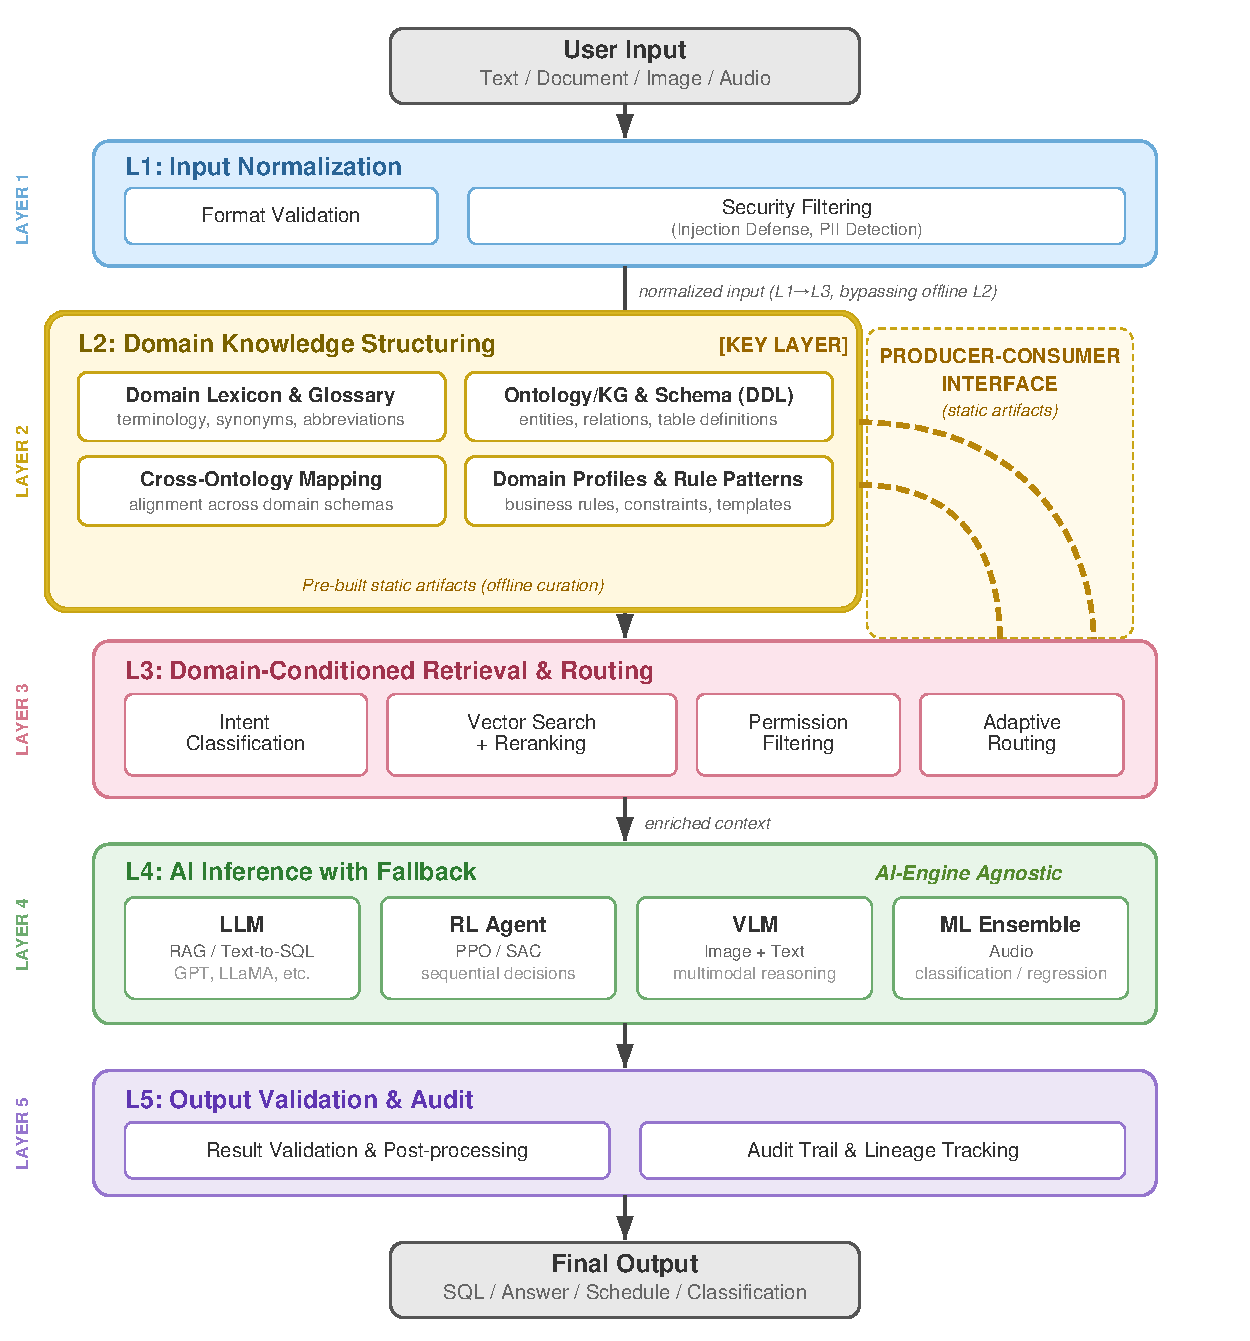
\includegraphics[width=\textwidth]{Fig2_DKAP_Architecture}
\caption{The five-layer Domain Knowledge Adaptation Pattern (DKAP). The defining dependency is the L2$\rightarrow$L3 producer--consumer interface: Layer~2 compiles \textit{static} domain artifacts (glossaries, ontologies, schemas, rule sets) offline, which Layer~3 consumes at query time for domain-conditioned retrieval and routing. Layer~1 normalizes input and Layer~5 validates output, while Layer~4 (AI inference) is engine-agnostic, accommodating LLMs, RL agents, VLMs, and ML ensembles.}
\label{fig:architecture}
\end{figure}

\subsection{Quantifying Domain Knowledge Complexity: DKS and RSS}

To characterize domain knowledge complexity across the twenty-nine systems---and to provide a lightweight, reusable descriptor for follow-up research---we define two heuristic rubrics with explicit checklist items: a Domain Knowledge Score (DKS) and a Retrieval Sophistication Score (RSS). We are precise about what these rubrics are and are not. They \textit{measure complexity}: the density and structural depth of explicit domain knowledge artifacts in source code. They are \textit{not} validated instruments for evaluating system quality or performance; a high DKS indicates a system encodes more structured domain knowledge, not that it is better.

We emphasize several caveats upfront. First, the rubrics are \textit{researcher-defined}; full human inter-rater validation has not yet been established and is a key limitation (Section~\ref{sec:limitations}). Second, the component weights (full rubric in the Supplemental Material) are based on the author's engineering judgment informed by observed variance across the 40+ systems, not on empirical optimization.

Third, we report a sensitivity analysis below showing that the main association holds under alternative weighting schemes. Fourth, DKS should be interpreted as a \textit{quasi-ordinal descriptive indicator} rather than a precise interval-scale measurement: comparisons between widely separated scores (a high-DKS versus a low-DKS system) are meaningful, whereas small differences (a gap of only a few points) fall within the rubric's judgment margin and should not be over-interpreted as a fine-grained ranking.

\subsubsection{Weight Rationale and Sensitivity}

DKS assigns higher weights (15 points) to components that exhibited the largest variance across systems in preliminary analysis---D1 (lexicon), D2 (ontology), D4 (schema), and D8 (regulatory)---and lower weights (10 points) to components with moderate variance. To assess robustness, we computed the DKS--Stages correlation under three alternative weighting schemes: (a) \textit{uniform weights} (all components $= 12.5$), (b) \textit{inverted weights} (swapping 15-point and 10-point components), and (c) \textit{rank-only} (ordinal ranking of each component). In all three cases, the Spearman correlation for the thirteen source-mined external systems (n$=$13---the paradigm-matched subset with independently verified source-code evidence, excluding the three unpaired externals Haystack, AutoGPT, and Rasa, which were author-scored only; see the Supplemental Material Table) remained significant and, if anything, equal to or higher than under the originally defined weighting ($\rho \geq 0.745$, $p < 0.004$; exact per-scheme values in the Supplemental Material), suggesting that the association is not an artifact of the specific weight assignment, and that the tiered D1--D8 weights are a descriptive rubric choice rather than a calibration tuned to this correlation. We provide the full sensitivity analysis, reproduction script, and per-component input data in the Supplemental Material. The reproduction script (\texttt{tools/sensitivity\_analysis.py}) was developed and verified with the assistance of Anthropic's Claude Code (\url{https://claude.ai}); the author independently reviewed the script and confirmed the reported correlations against the committed per-component data.

To assess whether the DKS--Stages association is driven by DKS or RSS individually, we computed each subscale's Spearman correlation with pipeline stage count separately, on the same sixteen external systems (n$=$16) used for the primary external-only correlation of Section~\ref{sec:external_validation}. DKS alone yields Spearman $\rho \approx 0.798$ ($p < 0.001$), closely tracking the composite DKS+RSS ($\rho = 0.789$), while RSS alone yields $\rho \approx 0.05$ ($p = 0.84$), which is not statistically significant. This characterizes how the composite descriptor behaves: it is effectively DKS-dominated, so the supporting DKS--Stages association (Section~\ref{sec:crossval}) is attributable to DKS, not RSS. This behavioral property justifies foregrounding DKS as the dominant subscale when describing domain knowledge complexity.

\subsubsection{Domain Knowledge Score (DKS)}

The DKS rubric (full per-component thresholds in the Supplemental Material) defines DKS $= \sum$(D1--D8), range [0, 100]. Each component score is anchored to \textit{countable code artifacts} extracted directly from source repositories. Concrete grounding examples: D1 is scored by counting glossary/lexicon entries (e.g., FinSQL: 1,170 column names across 78 financial tables $\rightarrow$ D1$=$10; MedRAG: no explicit glossary $\rightarrow$ D1$=$0). D2 is scored by examining ontology/graph structures (e.g., GraphRAG: full entity-relationship KG with hierarchical Leiden communities $\rightarrow$ D2$=$15; Pulse AI: no explicit KG or ontology $\rightarrow$ D2$=$0). D4 is scored by counting schema tables and FK constraints (e.g., FinSQL: 78 tables, 614 FKs $\rightarrow$ D4$=$10; EmotiVoice: YAML config with 105 lines $\rightarrow$ D4$=$8). D6 is scored by counting regex/rule patterns (e.g., Lineagis-AI: 18 injection defense patterns $\rightarrow$ D6$=$6). Complete per-system scoring evidence is provided in the Supplemental Material.

\subsubsection{Retrieval Sophistication Score (RSS)}

The RSS rubric (full thresholds in the Supplemental Material) defines RSS $= \sum$(R1--R5), range [0, 12]. We retain RSS as a separate record of retrieval-side sophistication for descriptive completeness; it is not part of the load-bearing complexity signal, which is DKS-dominated (Section~3.4.1).

\subsection{Complexity--Knowledge Association}

We examine whether pipeline stage count is associated with DKS and RSS scores. We use stage count as our primary complexity proxy because it is directly observable from the Architecture Mining Protocol (Step 2) and comparable across heterogeneous codebases regardless of programming language, team size, or deployment style. We acknowledge that stage count is a coarse metric: it is influenced by implementation style, team conventions, and production requirements (authentication, logging) that are orthogonal to domain knowledge. Alternative metrics such as lines of code (LOC), module count, or dependency graph depth could provide complementary perspectives; we chose stage count for its cross-language applicability and its direct correspondence to the data flow decomposition in our protocol. A system with 5 stages and a system with 18 stages differ meaningfully in architectural depth, even if some stages serve non-DKS purposes. We discuss this limitation further in Section~\ref{sec:limitations}.

The Supplemental Material lists all twenty-nine systems sorted by DKS+RSS. A positive trend is visible: systems with higher DKS+RSS scores tend to exhibit more pipeline stages, from MedRAG (DKS+RSS$=$10, 4 stages) through ClinicalRAG (DKS+RSS$=$94, 16 stages).


\subsection{Experimental Design}

To investigate the performance impact of L2 (Domain Knowledge Structuring), we conduct ablation experiments across three LLM-based domains (finance, healthcare, public procurement). The independent variable is the presence and depth of L2, controlled through three primary conditions (B1, B2, DKAP) plus a B1\_DDL diagnostic control (Table~\ref{tab:conditions}).

\textbf{Scope and limitations of this experiment.} This is an \textit{ablation study}, not a competitive benchmark. We do not claim that DKAP outperforms state-of-the-art Text-to-SQL systems (e.g., DIN-SQL~\citep{pourreza2023dinsql}, FinSQL~\citep{finsql}), which incorporate model-level optimizations (constrained decoding, schema linking, program synthesis) orthogonal to our architectural investigation. Rather, we isolate the effect of L2 by varying only the domain knowledge layer while holding all other variables constant (same LLM, same temperature, same prompt structure). B1 and B2 serve as controlled ablation conditions, not competitive baselines.

\textbf{Information fairness caveat.} We acknowledge that DKAP supplies strictly more information to the LLM than B2 (structured schema with semantic annotations vs.\ flat text chunks), which in turn supplies more than B1 (zero-shot). The expected direction of B1 $<$ B2 $<$ DKAP is therefore unsurprising in isolation. The purpose of this experiment is not to demonstrate that ``more information helps''---which is well-established---but rather to (a) measure the overall L2 benefit and decompose it into its information-completeness and structuring components, (b) examine how this benefit varies with domain knowledge complexity (DKS), and (c) probe its boundary conditions across domains---including a low-complexity domain where it is absent (an \textit{applicability threshold})---rather than assume a uniform cross-domain effect. The decomposition in (a)---holding information quantity constant while varying only its organization---is provided by the B2$'$ control in Section~\ref{sec:b2prime}.

\begin{table}[H]
\centering
\caption{Experimental Conditions}
\label{tab:conditions}
\footnotesize
\begin{tabularx}{\columnwidth}{@{}p{0.22\columnwidth}llX@{}}
\toprule
\textbf{Condition} & \textbf{L2} & \textbf{L3} & \textbf{Definition} \\
\midrule
B1: Vanilla LLM & OFF & Simple & Zero-shot prompt only. No few-shot examples. \\
B1\_DDL: Schema-only$^\ast$ & Off+ & None & Raw DDL (table/column names, types) only; no semantic annotations, no RAG. \\
B2: Flat-chunk RAG & Partial & BM25 & Flat chunks, no domain-aware segmentation. \\
DKAP (Proposed) & Full & Domain & Complete L1--L5 with structured L2 artifacts. \\
\bottomrule
\multicolumn{4}{@{}l}{\scriptsize $^\ast$B1\_DDL: Qwen3.6-27B-AWQ, finance subset ($n=28$, 3 runs). Not comparable to B1/B2/DKAP (Qwen3-32B-AWQ).} \\
\end{tabularx}
\end{table}

\subsection{Datasets and Metrics}

Table~\ref{tab:datasets} summarizes the evaluation datasets and metrics used across the three ablation domains.

\begin{table}[H]
\centering
\caption{Evaluation Datasets and Metrics. EX = execution accuracy (result-set match); EM = exact string match.}
\label{tab:datasets}
\footnotesize
\begin{tabularx}{\columnwidth}{@{}lXll@{}}
\toprule
\textbf{Domain} & \textbf{Dataset} & \textbf{Task} & \textbf{Metrics} \\
\midrule
Finance & Synthetic (from L2)$^\ddagger$ & Text-to-SQL & EX, EM \\
Healthcare & AIhub Clinical QA & Clinical SQL-QA & EX, EM \\
Public & KONEPS-style DB & Text-to-SQL & EX, EM \\
\bottomrule
\multicolumn{4}{@{}l}{\scriptsize $^\ddagger$Queries synthesized from the same L2 used in the ablation; see text.} \\
\end{tabularx}
\end{table}

For fair comparison, all conditions (B1, B2, DKAP) use the same base LLM (Qwen3-32B-AWQ via vLLM on dual H100 NVL GPUs) at temperature $= 0.0$ (greedy decoding), with batch composition held constant across reruns; our goal is to isolate the L2 effect without stochastic variance. Under this setup, the three reruns per condition produced identical outputs ($\sigma = 0.0$ observed). We note that temperature-0 decoding alone does not guarantee reproducibility under continuous batching: batch-size- and batch-composition-dependent reduction order in production serving can alter logits even at temperature zero~\citep{he2025nondeterminism}, so the $\sigma = 0.0$ we report is an empirical outcome of our fixed-batch-composition setup rather than a guarantee inherent to temperature-0 decoding in general. Temperature $>0$ experiments with multiple seeds, which provide additional statistical power, are reported in Sections~\ref{sec:b2prime} and~\ref{sec:crossmodel} ($n=5$ seeds and $n=10$ seeds across six model families, respectively). The finance benchmark comprises 50 Korean natural language questions of varying difficulty (13 Easy, 19 Medium, 18 Hard) targeting a realistic Korean financial card data warehouse schema with 5 tables.

\textbf{Query count note.} The three ablation domains use different query counts (Finance: 50Q; Healthcare: 40Q; Public: 25Q). The healthcare and public procurement sets were sized to match available benchmark queries rather than a pre-specified power target. Because standard errors scale as $1/\sqrt{n}$, the 25-query public procurement result carries the widest sampling uncertainty (95\% Wald confidence interval $\approx\pm$18.8pp for a binomial proportion at $n=25$) and should be interpreted with corresponding caution. Cross-domain EX comparisons between these benchmarks should therefore not be interpreted as quantitatively precise; their primary purpose is to identify qualitatively distinct operating regimes (Section~\ref{sec:cross_domain_summary}). We note that the finance test queries were synthesized from the same L2 knowledge base used in the DKAP condition---a design choice that ensures all queries genuinely require domain-specific schema knowledge, reflecting real-world deployment scenarios. All three conditions (B1, B2, DKAP) receive the identical test queries; what differs is each condition's access to the L2 knowledge: none for B1, unstructured for B2, and fully structured for DKAP. This design is therefore not circular but intentional for the ablation: it tests whether structured vs.\ unstructured access to known-necessary knowledge changes query performance.


\subsection{Computing Infrastructure and Data Preprocessing}
\label{sec:infra}

\textbf{Computing infrastructure.} The primary-model experiments (all B1, B1\_DDL, B2, B2$'$, and DKAP runs on Qwen3-32B-AWQ) were executed on a workstation running Ubuntu Linux (the distribution recalled by the author; the exact release version was not recorded) with two NVIDIA H100 NVL GPUs (96\,GB memory each), serving the model through vLLM~0.18.0 with tensor parallelism~$=2$, \texttt{max-model-len}~$=40960$, and \texttt{gpu-memory-utilization}~$=0.95$, under CUDA~12.8 and Python~3.11. Inference used vLLM's OpenAI-compatible \texttt{/v1/chat/completions} endpoint. The CPU model, system memory, and NVIDIA driver version were not recorded at experiment time and cannot be retrospectively retrieved, as the server belonged to the author's former employer and is no longer accessible. The recorded software stack (vLLM~0.18.0, CUDA~12.8, Python~3.11) and GPU configuration (2$\times$ NVIDIA H100 NVL, 96\,GB, tensor parallelism~$=2$, \texttt{max-model-len}~$=40960$, \texttt{gpu-memory-utilization}~$=0.95$) are the reproducibility-relevant parameters. The cross-model and cross-family experiments (Sections~\ref{sec:crossmodel} and~\ref{sec:limitations}) require no local GPU: they call the external model families through the OpenRouter API. The non-LLM reinforcement-learning ablation (Wheatley/JSSP) ran on a separate machine under Python~3.10 with PyTorch~2.2.0 (CUDA~12.1) and DGL~2.1.0. All statistical analyses and figure generation run on commodity CPU hardware using \texttt{numpy}, \texttt{scipy}, \texttt{pandas}, \texttt{scikit-learn}, and \texttt{matplotlib}; the exact package list is released with the code (\texttt{requirements.txt}), and full hardware/software versions are given in the Supplemental Material (``Experiment Scripts and Reproducibility'').

\textbf{Data preprocessing.} Each ablation domain is self-contained: the experiment script builds an in-memory SQLite database from an inline schema and synthetic seed records, then evaluates a fixed list of author-written natural-language/gold-SQL pairs. No external dataset is ingested at run time, so no record-level filtering, de-duplication, or de-identification was performed. The \emph{finance} set comprises 50 Korean questions (13 Easy, 19 Medium, 18 Hard) authored over a five-table synthetic Korean financial-card data-warehouse schema (member, transaction, and credit tables) and grounded in the same L2 knowledge base---schema DDL, business glossary, and column-transform rules---that the DKAP condition receives; each question is written to require domain-specific schema knowledge, so that a zero-shot model cannot resolve it from surface wording alone. The \emph{healthcare} set comprises 40 Korean questions over a clinical schema following the OMOP Common Data Model (patient, visit, condition, drug-exposure, and measurement tables), modeled on the AIhub Clinical QA domain and populated with synthetic records. The \emph{public-procurement} set comprises 25 Korean questions over a schema modeled on the KONEPS e-procurement system (bid-announcement, contractor, contract, and evaluation tables), likewise populated with synthetic records. No tokenization or text normalization is applied to the input questions: each is inserted verbatim into the condition-specific prompt template, which differs only in the L2 access it grants---none for B1, flat text chunks for B2, unstructured prose for B2$'$, and structured artifacts for DKAP. On the output side, each model response has its Qwen3 \texttt{<think>} reasoning block removed by a regular expression before scoring, and the generated SQL is normalized (lower-casing, whitespace collapsing, and trailing-semicolon removal) prior to execution-accuracy comparison. The internal industrial systems analyzed in the cross-validation are proprietary: only their derived, non-identifying architecture scores (DKS, RSS, and stage counts) are used, and no raw internal code or data is redistributed.


%% ============================================================
%%  SECTION 4: RESULTS
%% ============================================================
\section{Results}

\subsection{Finance Domain Results}
\label{sec:finance_results}

Table~\ref{tab:finance_results} presents the execution accuracy (EX) and exact match (EM) results for the finance Text-to-SQL task.

\begin{table}[H]
\centering
\caption{Finance Text-to-SQL Results (Qwen3-32B-AWQ, 50 queries; the ``$\times$3'' denotes three reruns at temperature~$0$ with fixed batch composition, which produced identical outputs ($\sigma=0$ observed)---this is an empirical result, not a claim about stability under sampling). EX = execution accuracy (result-set match); EM = exact string match; EXEC = fraction of generated SQL that runs without error (syntactic validity).}
\label{tab:finance_results}
\footnotesize
\begin{tabularx}{\columnwidth}{@{}Xrrrr@{}}
\toprule
\textbf{Condition} & \textbf{EX\%} & \textbf{EM\%} & \textbf{EXEC\%} & \textbf{Lat.(ms)} \\
\midrule
B1: Vanilla LLM ($\times$3)  & 0.0  & 0.0 & 0.0   & 970  \\
B2: Flat-chunk RAG ($\times$3) & 54.0 & 4.0 & 84.0  & 1207 \\
DKAP (Proposed) ($\times$3)  & 80.0 & 4.0 & 100.0 & 1324 \\
\bottomrule
\end{tabularx}
\end{table}

Three key findings emerge. First, B1 fails outright without domain knowledge: B1 (zero-shot) achieves 0.0\% execution accuracy across all difficulty levels, generating SQL that references non-existent tables. This is a \textit{floor} result---the queries require multi-table joins that a zero-shot model cannot resolve without any schema (we revisit this floor effect in the Supplemental Material)---confirming that even a 32B-parameter model cannot bridge the semantic grounding gap without domain context.

Second, partial L2 (B2) helps significantly but degrades with complexity. B2 achieves 92.3\% EX on Easy queries but drops to 63.2\% on Medium and 16.7\% on Hard. The flat-chunk retrieval supplies table names and column lists but lacks the additional domain knowledge (join conditions, value-domain mappings, semantic glossary) needed for complex query synthesis---knowledge that, as Section~\ref{sec:b2prime} shows, drives most of the gain whether supplied as structured artifacts or as plain prose.

Third, the full DKAP condition improves over B2 at every difficulty level. DKAP achieves 100.0\% EX on Easy ($+$7.7pp vs.\ B2), 89.5\% on Medium ($+$26.3pp), and 55.6\% on Hard ($+$38.9pp). The improvement gap over B2 \textit{widens monotonically with query complexity} ($+$7.7pp $\rightarrow$ $+$26.3pp $\rightarrow$ $+$38.9pp), a pattern we refer to descriptively as the \textit{widening gap}. We caution against over-reading this gap as evidence of structuring: the B2-vs-DKAP contrast varies \textit{both} the amount of domain knowledge and its structure, so the widening gap alone cannot attribute the benefit to structural organization rather than to information completeness. The information-matched control in Section~\ref{sec:b2prime} (B2$'$) isolates exactly this confound, and shows that information completeness is the primary driver while structural organization contributes a smaller, difficulty-dependent precision gain. Notably, DKAP achieves 100.0\% execution rate (all generated SQL is syntactically valid), compared to 84.0\% for B2.

\textbf{B1\_DDL control: isolating schema structure from domain knowledge.} A natural concern is whether B1's 0.0\% EX reflects the absence of \textit{any} schema information, rather than the absence of structured domain knowledge specifically. To address this, we ran a B1\_DDL condition that supplies the raw DDL schema (CREATE TABLE statements: column names and data types only, no semantic annotations, no join rules, no value-domain mappings, no retrieval). We ran this diagnostic later than the main ablation and used the then-current evaluation-time model (Qwen3.6-27B-AWQ) on a representative 28-query subset (13 Easy, 9 Medium, 6 Hard), 3 runs at temperature~0; because the base model differs from B1/B2/DKAP, we interpret only its qualitative difficulty gradient, not its absolute values (see below). B1\_DDL achieves 63.1\% overall EX (Easy: 92.3\%, Medium: 51.9\%, Hard: 16.7\%). Two conclusions follow. First, the B1=0\% result is consistent with a genuine zero-shot limitation: schema structure alone produces a $+$63.1pp improvement over zero-shot, so B1=0\% is not an artifact of the task being unsolvable---it reflects the LLM's inability to infer schema structure from parametric knowledge alone. Second, the B1\_DDL difficulty gradient (Easy 92.3\%$\to$Medium 51.9\%$\to$Hard 16.7\%) mirrors the widening-gap direction, suggesting that the penalty for missing semantic annotations and join rules is largest for complex multi-join queries; this is consistent with controlled prompt-format studies showing that schema serialization choices materially affect Text-to-SQL accuracy~\citep{chang2023prompt}. We note that B1\_DDL uses a different base model than B1/B2/DKAP, so absolute cross-condition comparisons require caution; the qualitative pattern---schema structure alone being insufficient for hard queries---is the primary finding.

\subsection{Healthcare Domain Results}

The healthcare results confirm the cross-domain pattern for execution accuracy: B1 (2.5\%) $\ll$ B2 (57.5\%) $\ll$ DKAP (70.0\%). DKAP's improvement over B2 is $+$12.5pp overall, smaller than finance ($+$26.0pp), consistent with the OMOP CDM being a more standardized and LLM-familiar schema structure. DKAP achieves 100.0\% execution rate and dominates B2 on both Easy ($+$25.0pp) and Medium ($+$14.3pp) queries; Hard query EX is identical (35.7\% each).

\textbf{EM reversal on Easy queries.} The healthcare results (Supplemental Material) reveal an apparent anomaly: DKAP's overall EM (7.5\%) is \textit{lower} than B2's (12.5\%), despite DKAP achieving higher EX. Difficulty-stratified analysis isolates the reversal entirely to Easy queries, where DKAP EM$=$8.3\% versus B2 EM$=$25.0\%; Medium and Hard EM are identical between conditions ($\leq$14.3\% each). The mechanism is structural: DKAP's L2 artifacts encode full OMOP CDM joins---traversing \texttt{concept}, \texttt{drug\_era}, and \texttt{measurement} tables through FK chains and vocabulary concept IDs---and L3 injects these join paths into generated SQL. The reference queries in the AIhub Clinical QA benchmark were written against a flatter clinical schema, so even a semantically correct DKAP query (one that executes and returns the right rows) does not match the reference token-for-token. B2's simpler flat-chunk retrieval produces SQL that more closely resembles the reference pattern on straightforward Easy queries, yielding higher EM even when it executes less reliably (EXEC 87.5\% vs.\ 100.0\%). In other words, the EM gap reflects a structural \textit{mismatch between DKAP's CDM-compliant query generation and the reference SQL vocabulary}, not an accuracy deficit. This finding highlights a known limitation of string-based EM as an evaluation metric for domain-adapted SQL systems: EM penalizes semantically equivalent queries that differ in join strategy or vocabulary identifier style.

Notably, DKAP (739\,ms) exhibits \textit{lower} latency than B2 (1{,}151\,ms), an apparently counterintuitive result. We attribute this to domain-aware L2 pre-filtering: DKAP's structured ontology and schema map narrow the retrieval scope before the vector search stage (L3), substantially reducing the number of candidate chunks and thus retrieval time; B2's unstructured BM25 search over the full corpus is comparatively slower. We report this as a single-domain observation rather than a general benefit: DKAP reduced latency only in healthcare, whereas it was slightly \textit{slower} than B2 in finance ($1{,}324$ vs.\ $1{,}207$\,ms) and public procurement ($697$ vs.\ $604$\,ms). Any throughput effect of L2 pre-filtering is therefore domain-specific and would require controlled isolation (corpus size, caching, top-$k$ held fixed) to establish.

\subsection{Public Procurement Results}

The public procurement domain (its ablation-specific L2 knowledge score $\mathrm{DKS}_{\mathrm{L2}}=8$, defined in Section~\ref{sec:cross_domain_summary}, is the lowest of the three ablation L2 artifact sets) yields a null result for semantic accuracy (Supplemental Material): DKAP and B2 achieve identical EX (64.0\%) and EM (8.0\%). Rather than viewing this as a failure of DKAP, we interpret it as evidence of an \textit{applicability threshold}: with only 6 tables, no foreign key constraints, and self-descriptive Korean column names, the domain knowledge gap is minimal---the LLM's pre-training already covers procurement vocabulary sufficiently.

This suggests that DKAP's architectural investment in L2 yields returns only when domain knowledge complexity exceeds a certain level. Below this threshold, simpler approaches (flat-chunk RAG) may be equally effective, which is itself a useful practical finding. The only observed difference is syntactic validity (EXEC: 96.0\% vs.\ 84.0\%), suggesting that structured schema annotations improve SQL well-formedness even when semantic accuracy has converged. We present this result transparently as a boundary condition that strengthens, rather than undermines, the DKS--benefit relationship.

\subsection{Cross-Domain Summary}
\label{sec:cross_domain_summary}

\begin{table}[H]
\centering
\caption{Cross-Domain Comparison (Execution Accuracy \%). Three case studies exploring DKS--benefit boundary conditions; not a statistical proof of a cross-domain trend ($n=3$ insufficient for regression).}
\label{tab:cross_domain}
\footnotesize
\begin{tabularx}{\columnwidth}{@{}Xrrrrr@{}}
\toprule
\textbf{Domain} & \textbf{B1} & \textbf{B2} & \textbf{DKAP} & $\Delta$ & \textbf{DKS}$^{*}$ \\
\midrule
Finance (50Q)    & 0.0 & 54.0 & 80.0 & $+$26.0pp & 72 \\
Healthcare (40Q) & 2.5 & 57.5 & 70.0 & $+$12.5pp & 65 \\
Public (25Q)     & 0.0 & 64.0 & 64.0 & $+$0.0pp  & 8 \\
\bottomrule
\multicolumn{6}{@{}p{\columnwidth}@{}}{\scriptsize $\Delta$=DKAP$-$B2 (pp). $^{*}$Ablation L2 DKS (per-ablation L2 artifact set, not the system-level total; cf.\ the Supplemental Material 29-system table).} \\
\end{tabularx}
\end{table}

\textbf{Observed trend: the L2 benefit tracks domain complexity.} Across the three domains, the DKAP (L2) benefit over flat-chunk retrieval increases monotonically with an \textit{ablation-specific} L2 knowledge score ($\mathrm{DKS}_{\mathrm{L2}}$, scored from the released L2 prompts prior to and independently of the ablation outcomes, so it is auditable and not fitted): high-complexity finance ($\mathrm{DKS}_{\mathrm{L2}}{=}72$) gains $+$26.0pp, mid-complexity healthcare ($65$) $+$12.5pp, and low-complexity public procurement ($8$) $+$0.0pp. This gives DKS a concrete operational reading---a \textit{descriptive indicator of when knowledge structuring is worthwhile}: where domain knowledge is dense, compiling it into L2 artifacts pays off; where the schema is shallow and already covered by pretraining, it adds nothing semantic (only syntactic validity, EXEC $96.0\%$ vs.\ $84.0\%$). We present this as an observed trend across three boundary-condition cases---not a fitted law---and bound it immediately below.

\textbf{Scope caveat.} We emphasize that Table~\ref{tab:cross_domain} presents three case studies, not a statistically powered cross-domain analysis. Three data points are insufficient to establish a regression trend: any three distinct values can be ordered monotonically by construction. We therefore make no claim that the observed ordering (finance $>$ healthcare $>$ public) constitutes evidence of a general DKS--benefit law. Instead, we interpret these three cases as \textit{boundary condition explorations}: (1) a high-DKS domain where L2 yields large benefits, (2) a mid-DKS domain where benefits are moderate, and (3) a low-DKS domain where L2 yields no semantic benefit---three qualitatively distinct operating regimes that motivate the applicability threshold hypothesis. Quantitative validation of the DKS--benefit relationship requires $n \geq 5$ domains with independent DKS assessment, which we identify as priority future work.

Because the B2$\to$DKAP contrast changes both the amount of domain knowledge and its structure, this cross-domain comparison cannot, by itself, separate the roles of information completeness and structural organization; it is best read as a boundary-condition signal of how the \textit{combined} L2 benefit scales with domain complexity. That separation is addressed directly, for the finance domain, by the information-matched control (B2$'$) in Section~\ref{sec:b2prime}, which attributes the bulk of the benefit to information completeness and a smaller, difficulty-dependent share to structural organization. A qualitative cross-paradigm RL scheduling illustration is provided in the Supplemental Material.

\subsection{Information Completeness vs.\ Structural Organization}
\label{sec:b2prime}

The B2--DKAP comparison confounds two factors: DKAP supplies both \textit{more} information and \textit{better-structured} information than B2. To disentangle these, we introduce a B2$'$ condition that supplies the same domain knowledge as DKAP---DDL, join rules, value-domain mappings, semantic glossary---but written as unstructured narrative prose instead of structured tables and annotations.

We authored the B2$'$ prose with content limited to the same factual elements present in the DKAP L2 artifacts; narrative prose nonetheless unavoidably introduces incidental reasoning cues absent from DKAP's bare tables (e.g., explicit join-condition reminders), a directional caveat we detail below and in Supplemental Material S2. Token counts were verified to match within 2\% (DKAP: ${\sim}$1{,}960 tokens vs.\ B2$'$: ${\sim}$1{,}920 tokens) to control for information volume.

This design follows the logic of content-controlled representation studies: concurrent work by \citet{zhang2026samecontent} isolates the effect of representation in table question answering by holding informational content fixed while varying its structure, reaching a convergent conclusion---that the benefit of structure is method- and difficulty-dependent rather than uniform; relatedly, \citet{sui2024table} find that LLMs' comprehension of structured tables is itself sensitive to serialization, underscoring that tabular form is not automatically advantageous over equivalent prose.

We flag one \textit{directional} caveat: the B2$'$ prose incidentally carries elaborative reasoning cues (e.g., explicit join-condition reminders) that DKAP's bare tables lack, which advantages B2$'$ and therefore biases the structuring contrast (DKAP$-$B2$'$) \textit{downward}. Two consequences follow. First, our near-zero structuring result should be read as ``tabular structuring offers no detectable advantage over information-matched prose,'' not as ``structure is intrinsically useless''---a true structuring benefit, if any, is only partially masked by the prose's free cues. Second, and more importantly, because this bias runs \textit{against} DKAP, it is unlikely to explain the completeness gain (B2$'-$B2): the robust, cross-model completeness finding is conservative with respect to this confound, not produced by it. Readers should interpret the B2$'\!\to\!$DKAP comparison with this directional caveat.

\begin{table}[H]
\centering
\caption{Information Completeness vs.\ Structuring (Finance, 50Q, temp$=$0.0)}
\label{tab:b2prime}
\footnotesize
\begin{tabularx}{\columnwidth}{@{}Xrrrr@{}}
\toprule
\textbf{Condition} & \textbf{EX\%} & \textbf{Easy} & \textbf{Med} & \textbf{Hard} \\
\midrule
B2 (flat-chunk RAG) & 54.0 & 92.3 & 63.2 & 16.7 \\
B2$'$ (prose, same info) & 80.0 & 92.3 & 84.2 & 66.7 \\
DKAP (structured)   & 80.0 & \textbf{100.0} & \textbf{89.5} & 55.6 \\
\bottomrule
\end{tabularx}
\end{table}

Three findings emerge from Table~\ref{tab:b2prime}. First, the primary driver of the B2$\to$DKAP improvement is \textit{information completeness}: both B2$'$ and DKAP achieve 80.0\% overall EX, a $+$26.0pp gain over B2, confirming that providing complete domain knowledge is necessary and largely sufficient for the overall accuracy improvement.

Second, structural organization yields measurable \textit{precision advantages} at lower difficulty levels: DKAP outperforms B2$'$ on Easy ($+$7.7pp) and Medium ($+$5.3pp) questions, where correct table--column mapping is the primary challenge. On Hard queries the direction \textit{reverses}---B2$'$ reaches 66.7\% versus DKAP's 55.6\% ($-$11.1pp)---so restricting the structuring contrast to Easy/Medium is, if anything, favorable to DKAP; we report this reversal rather than hide it (Hard performance is gated by multi-step reasoning the tables do not encode). We emphasize that these per-difficulty deltas rest on small per-bin counts (13 Easy, 19 Medium) on a single deterministic model and are not individually significant; the cross-model panel of Section~\ref{sec:crossmodel} is the inferential basis, and it shows this advantage does not generalize. Error analysis of the two Hard questions where B2$'$ succeeds and DKAP fails (Q21, Q29) reveals that DKAP's errors are column-omission and aggregation-type mismatches---not systematic failures of the structured approach.

Third, stochastic robustness testing (temperature$=$0.3, 5 runs; per-run values: B2$=[52,56,56,56,58]$, B2$'=[78,78,80,76,78]$, DKAP$=[80,78,78,78,78]$) provides a directionally consistent picture:

\textbf{Statistical caveat on $\sigma$.} With only $n=5$ runs, bootstrap 95\% confidence intervals for $\sigma$ are wide and all include zero (Supplemental Material), meaning the observed ordering (DKAP $<$ B2$'$ $<$ B2 in variance) is directionally consistent but not statistically significant at this sample size. We report these intervals transparently rather than claiming confirmed stability differences. The rank ordering of mean EX\% (DKAP $\approx$ B2$' >$ B2) is, however, stable across all five runs with zero crossings, providing stronger evidence for the accuracy pattern than for the variance pattern. Increasing to $n \geq 20$ runs is identified as priority follow-up to establish the stability claim.

DKAP exhibits the lowest output variance ($\sigma = 0.9$, range $[78,80]$) across all conditions; whether this reflects a genuine structural stabilization effect or sampling variability cannot be determined from $n=5$ runs alone. We therefore qualify our interpretation: \textit{information completeness is the confirmed primary driver of the B2--DKAP gap ($+$26.0pp, stable across all 5 runs); structural organization yields measurable secondary gains in schema-mapping precision on Easy/Medium queries ($+$5.3--7.7pp on this base model; but see the cross-model test in Section~\ref{sec:crossmodel}), and a directionally lower variance ($\sigma=0.9$ vs.\ $1.4$) that requires larger-$n$ confirmation.}

\subsection{Cross-Model Generalization}
\label{sec:crossmodel}

The decomposition above was measured on a single base model (Qwen3-32B-AWQ). To test whether it generalizes---and to address the concern that the secondary structuring gain might be model-specific---we rerun the finance B2 / B2$'$ / DKAP ablation across six independent, lineage-distinct model families accessed via OpenRouter (OpenAI GPT-5.4, Anthropic Claude Sonnet~4.6, Google Gemini~3.1~Pro, DeepSeek~V3.2, Alibaba Qwen3.6-27B, and Mistral Medium~3.5)\footnote{The cross-family reliability study (Section~\ref{sec:limitations}) uses seven judge lineages to maximize evaluator diversity, whereas the ablation uses six (GLM-5.2 excluded) as the systems under test; the two studies serve different roles and need not share an identical model set.}, each at temperature~$0.3$ with ten seeds ($50$ questions $\times\,6$ models $\times\,3$ conditions $\times\,10$ seeds $=9{,}000$ runs). Table~\ref{tab:crossmodel} reports the per-family numbers, and Fig.~\ref{fig:teaser} visualizes the same data as a three-bar decomposition separating each family's completeness gain (B2$\rightarrow$B2$'$) from its structuring gain (B2$'\rightarrow$DKAP).

\begin{table}[H]
\centering
\caption{Cross-model finance ablation (six independent model families, ten seeds each, temperature$=$0.3, execution accuracy \%). The completeness gain (B2$'-$B2) replicates across all six families; the structuring gain (DKAP$-$B2$'$, Easy$+$Medium) is not distinguishable from zero.}
\label{tab:crossmodel}
\footnotesize
\begin{tabularx}{\columnwidth}{@{}Xrrr@{}}
\toprule
\textbf{Model} & \textbf{B2} & \textbf{Compl.} & \textbf{Struct.} \\
 & & \textbf{B2$'\!-$B2} & \textbf{DKAP$-$B2$'$} \\
\midrule
OpenAI GPT-5.4 & 65.4 & $+$18.0 & $-$0.9 \\
Anthropic Claude Sonnet 4.6 & 64.6 & $+$18.8 & $+$1.2 \\
Google Gemini 3.1 Pro & 60.4 & $+$9.8 & $+$4.4 \\
DeepSeek V3.2 & 53.8 & $+$21.8 & $+$0.3 \\
Alibaba Qwen3.6-27B & 60.0 & $+$14.6 & $+$1.9 \\
Mistral Medium 3.5 & 57.2 & $+$22.2 & $-$2.5 \\
\midrule
\textbf{Mean} & & \textbf{+17.5} & \textbf{+0.7} \\
\multicolumn{4}{@{}l}{\scriptsize Structuring 95\% CI (both incl.\ 0): pooled $[-1.0,3.0]$, family $[-0.95,2.50]$.} \\
\bottomrule
\end{tabularx}
\end{table}

Two findings stand out. First, the \textit{completeness} gain (B2$'-$B2) is robust and universal: $+$17.5pp on average and positive for all six families ($+$9.8 to $+$22.2pp), confirming across independent models that supplying complete domain knowledge---in any form---is the primary driver of accuracy.

Second, the \textit{structuring} gain (DKAP$-$B2$'$ on Easy/Medium), with information held fixed, is \textit{not} distinguishable from zero across models: mean $+$0.7pp, with two of six families negative (pooled $95\%$ bootstrap CI $[-1.0, +3.0]$ over the per-family, per-query Easy/Medium differences). Because a cross-family claim should treat the model family as the replication unit, we also cluster-bootstrap the six family-level gains; this gives a consistent $95\%$ CI of $[-0.95, +2.50]$ (Student-$t$ $[-1.8, +3.2]$), again including zero. Notably, even a newer Qwen (Qwen3.6-27B) yields only $+$1.9pp, so the $+$5.3--7.7pp gain seen on the original Qwen3-32B does not generalize even within the Qwen lineage.

We therefore read the structuring effect as \textit{model-specific and near-null on modern models}: once the necessary information is complete, presenting it as structured tables rather than equivalent prose hits a performance ceiling and confers no reliable additional accuracy on capable models. This \textit{sharpens} rather than weakens the paper's thesis---completeness, not structure, is the robust cross-model driver. We confine the cross-model structuring null to finance, the only domain with a B2$'$ control; healthcare and public procurement isolate the combined L2 benefit but not its structuring component, so we make no claim that the structuring null itself generalizes across domains. Replication of the B2$'$ decomposition on an independent, externally-sourced benchmark is priority future work.

It also \textit{replicates}, at the system-architecture level and with cross-model statistical bounds (six families, $9{,}000$ runs), the single-model, prompt-level observation of \citet{maamari2024death} that strong reasoning-capable models absorb complete schema information largely regardless of its serialization: our contribution is not the direction of the effect but its establishment as a controlled, cross-model architectural result rather than a one-model finding.

\begin{figure}[tp]
\centering
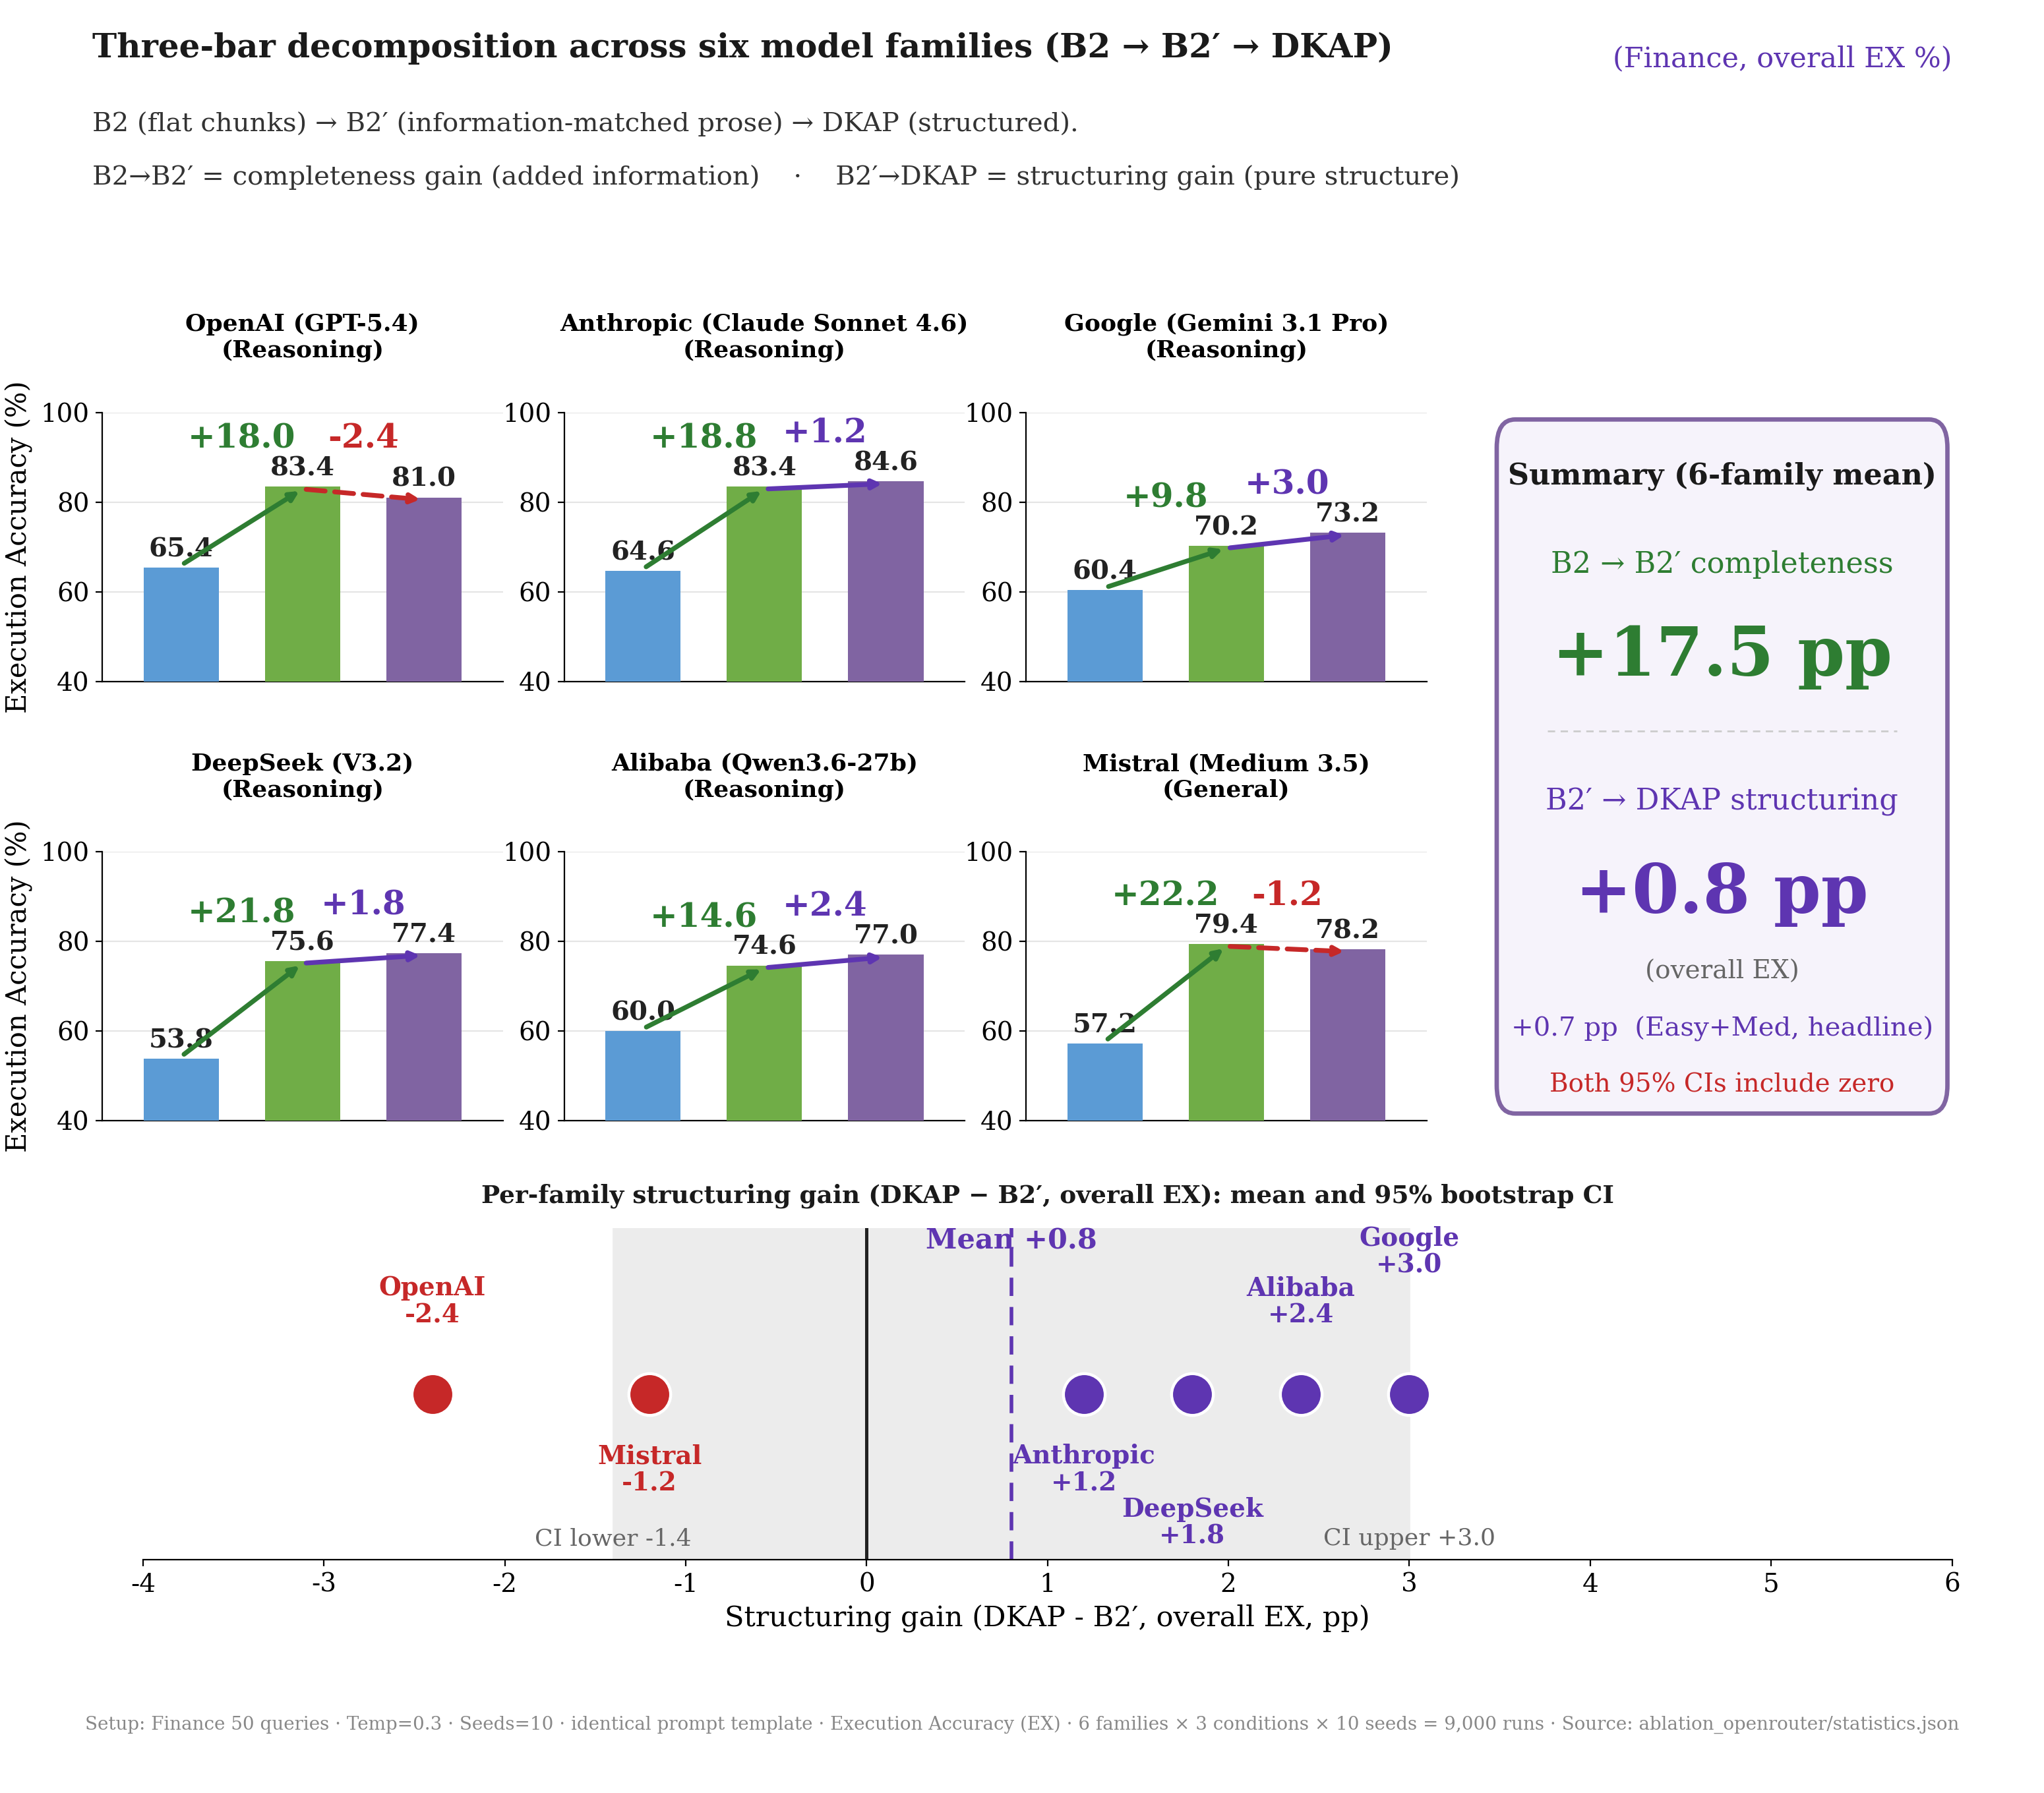
\includegraphics[width=\textwidth]{teaser_3bar_decomposition_en.png}
\caption{Three-bar decomposition of the finance ablation across six independent model families (execution accuracy, \%). For each family the bars show B2 (flat chunks) $\rightarrow$ B2$'$ (information-matched prose) $\rightarrow$ DKAP (structured): the green arrow isolates the \textit{completeness} gain (adding information) and the second arrow the \textit{structuring} gain (pure structure, with information held fixed). The completeness gain is large and positive for all six families ($+$17.5pp mean), whereas the structuring gain (bottom strip) scatters around zero with mixed signs: the Easy$+$Medium headline subset gives $+$0.7pp (pooled $95\%$ CI $[-1.0, 3.0]$; cf.\ Table~\ref{tab:crossmodel}), and the overall-EX variant gives $+$0.8pp (family-level Student-$t$ $95\%$ CI $[-1.4, 3.0]$, $n=6$ families)---both including zero. Source data: \texttt{ablation\_openrouter/statistics.json}.}
\label{fig:teaser}
\end{figure}


%% ============================================================
%%  SECTION 5: DISCUSSION
%% ============================================================

\section{Discussion}

\subsection{Why Does L2 Absence Degrade Performance?}

When L2 is absent (B1), the LLM interprets domain terms via its general pre-training distribution---``account'' as a general concept rather than \texttt{account\_table.account\_id}, or ``Metformin'' as a generic drug rather than \texttt{drug\_concept\_id = 1503297} in the OMOP CDM vocabulary. L2 bridges this semantic grounding gap, which exists regardless of the AI engine: RL agents need domain-structured rewards, ML classifiers domain-profiled features, and VLMs domain-contextualized prompts.

\subsection{Why Might DKAP Appear Across Different AI Engines?}

A possible explanation for the cross-paradigm consistency is that every AI system requires domain context as input (LLMs need grounded prompts, RL agents domain-structured rewards, ML classifiers domain-profiled features), so L2 (context preparation) and L3 (context delivery) form a separation of concerns that emerges whenever domain knowledge is non-trivial. We note this explanation is post-hoc: the five-layer decomposition may also reflect common software-engineering practice (separation of concerns, layered design) rather than an AI-specific phenomenon.

\textbf{Falsifiability and counter-examples.} Is the DKAP observation falsifiable? We propose that a system \textit{disconfirms} DKAP if the Architecture Mining Protocol finds no code preparing static domain artifacts consumed by downstream retrieval or routing---whether as a dedicated stage or embedded within one (the code-level criterion of Section~3.2). Concretely, disconfirming cases would be (i) domain knowledge embedded directly in model weights with no runtime injection point, or (ii) retrieval over raw documents with no domain-aware pre-filtering, indexing, or segmentation. Candidate counter-examples exist in our considered-but-excluded inventory (Supplemental Material)---e.g., a thin zero-shot API wrapper or a bare speech-to-text wrapper would score L2$=$0. That all twenty-nine \textit{selected} systems exhibit DKAP must be read against our inclusion criteria, which required non-trivial domain adaptation; validating the falsifiability boundary on systems designed without explicit domain structuring is priority future work.

\subsection{Association Between Domain Knowledge and Pipeline Complexity}

As a \textit{supporting observation}---secondary to the ablation results of Section~\ref{sec:finance_results}---we examine whether the complexity characterized by DKS+RSS tracks pipeline depth across our systems. The positive association between DKS+RSS and pipeline stage count across the twenty-nine systems (the Supplemental Material 29-system table) warrants careful interpretation. Among the sixteen independently developed external systems, both parametric and non-parametric tests reach significance: Pearson $r = 0.857$ (95\% CI [0.63, 0.95], $p < 0.001$) and Spearman $\rho = 0.789$ ($p < 0.001$), with $R^2 = 0.734$ (adjusted $R^2 = 0.715$) (scatter plot in the Supplemental Material). This external-only analysis reduces (but does not eliminate) the confound of shared organizational design biases. Across all twenty-nine systems, the association is strong: Pearson $r = 0.868$ ($p < 0.001$, $R^2 = 0.753$) and Spearman $\rho = 0.873$ ($p < 0.001$).

\textbf{Correlation vs.\ causation.} We emphasize that this association does not establish a causal direction. An equally plausible alternative explanation is that complex systems (due to production requirements, regulatory compliance, team size) naturally accumulate both more domain artifacts and more pipeline stages, with a common cause driving both. Our data cannot distinguish between ``domain knowledge complexity drives architecture depth'' and ``both are consequences of system maturity or deployment requirements.'' The external-only analysis partially mitigates this concern (external systems lack production infrastructure), but the sample size ($n = 16$) limits the strength of this argument.

The five non-LLM systems---Wheatley~\citep{wheatley} (RL+GNN, 35, 8 stages), SpeechBrain~\citep{speechbrain} (ASR/TTS, 41, 8), AudioCraft~\citep{audiocraft} (Transformer~LM, 46, 7), EmotiVoice~\citep{emotivoice} (BERT+TTS, 50, 8), and Rasa (BERT+ML, 44, 8)---fall within the regression trend, providing some evidence that the association is not LLM-specific.

Two informative contrasts emerge. First, the \textit{framework contrast}: LlamaIndex~\citep{llamaindex} (DKS$=$20) and CrewAI (DKS$=$15) are generic frameworks with intentionally low built-in domain knowledge, whereas EmotiVoice (DKS$=$47) and GraphRAG (DKS$=$57) encode rich domain artifacts. Second, the \textit{compactness contrast}: MetaGPT~\citep{metagpt} (DKS$=$37, 6 stages) achieves high knowledge density via structured roles and workflow templates, showing role-based architectures can encode domain knowledge with fewer stages and partially \textit{weakening} the linear DKS--Stages relationship.

\subsection{Tentative Design Hypotheses}

Based on the patterns observed in our sample, we offer the following \textit{hypotheses} (not prescriptions) for practitioners to evaluate in their own contexts: (1) Early investment in domain knowledge structuring (L2) may reduce downstream integration complexity. (2) Separating knowledge structuring (L2) from retrieval routing (L3) may improve maintainability by isolating domain-specific artifacts from execution logic. (3) Treating the AI inference layer (L4) as a replaceable component may facilitate technology migration. (4) Domains with richer domain knowledge may require deeper pipelines. These suggestions are grounded in our observations but have not been validated through controlled deployment studies. We cannot rule out that the observed consistency across our twenty-nine systems reflects selection bias or common engineering conventions rather than a design principle.

\subsection{External Validation --- DKS Distribution Analysis \texorpdfstring{($n=16$)}{(n=16)}}
\label{sec:external_validation}

To assess generalizability beyond the internal system portfolio, we analyze sixteen independently developed external open-source systems using the same Architecture Mining Protocol (Section~3.2). The Supplemental Material reports the DKS+RSS scores, pipeline stages, and LOC for all sixteen external systems.

\textbf{LOC as a supplementary complexity metric.} The Supplemental Material external-systems table also reports Python LOC and file counts. The DKS+RSS--LOC correlation is weak and non-significant (Spearman $\rho = 0.23$, $p = 0.45$), inflated by framework and research systems with large code volume but modest domain knowledge (CrewAI, LlamaIndex, DeepTutor~\citep{deeptutor}, MetaGPT); excluding frameworks, it strengthens ($\rho = 0.66$, $p = 0.03$, $n = 11$). Stage count and LOC thus capture different aspects of complexity.

Several further observations emerge (the DKS+RSS--Stages correlation and the paradigm-matched comparison are detailed in the surrounding subsections):

\textbf{Effect size and robustness of the association.} Beyond the external-only correlation reported above ($r = 0.857$, 95\% CI [0.63, 0.95]; $\rho = 0.789$), the linear fit (Stages $\approx 0.09 \times$ DKS+RSS $+ 4.0$) implies that each ${\sim}11$-point increase in DKS+RSS corresponds to one additional pipeline stage.

\textbf{Influence analysis.} To assess whether the association is driven by one or two outlying systems, we computed Cook's distance for all sixteen external systems. Only MedRAG~\citep{medrag} (Cook's $D = 0.365$) exceeds the conventional $4/n = 0.25$ threshold; no system exceeds the more conservative $F_{0.5}(2, 14) = 0.729$ criterion. Leave-one-out (LOO) Pearson $r$ ranges from $0.799$ (excluding MedRAG) to $0.896$ (excluding MetaGPT), remaining significant ($p < 0.001$) in all sixteen LOO iterations. LOO Spearman $\rho$ ranges from $0.742$ to $0.848$, likewise significant throughout. The association is therefore not attributable to any single system.

\textbf{Statistical power.} We report only the \textit{a priori} sensitivity: at $n = 16$, $\alpha = 0.05$ (two-tailed), and $80\%$ power, the minimum detectable correlation is $r = 0.651$, which the observed point estimate ($r = 0.857$) exceeds. (We avoid post-hoc ``achieved power'' computed from the observed effect, as it is a monotone restatement of the $p$-value and not independently informative.)

\subsection{Internal--External Cross-Validation}
\label{sec:crossval}

To validate that DKAP captures a genuine architectural pattern rather than an artifact of development context, we perform pairwise cross-validation between internal and external systems sharing the same AI paradigm. Table~\ref{tab:crossval} presents all thirteen paradigm-matched pairs.

\begin{table}[H]
\centering
\caption{Paradigm-Matched Cross-Validation (13 Pairs)}
\label{tab:crossval}
\footnotesize
\begin{tabularx}{\columnwidth}{@{}lXrrXrr@{}}
\toprule
\textbf{Paradigm} & \textbf{Ext.} & \textbf{Tot} & \textbf{St} & \textbf{Int.} & \textbf{Tot} & \textbf{St} \\
\midrule
Hlth RAG    & MedRAG      & 10 &  4 & ClinicalRAG & 94 & 16 \\
Doc RAG     & LlamaIdx    & 27 &  6 & ex-GPT      & 45 &  7 \\
Txt2SQL     & BIRD-SQL    & 29 &  7 & Lineagis-AI & 90 & 12 \\
DomFT       & FinSQL      & 41 &  7 & nama        & 46 &  8 \\
RL+Sched    & Wheatley    & 35 &  8 & ShipSched   & 59 &  9 \\
Speech      & SpchBrain   & 41 &  8 & babel-aud   & 72 &  8 \\
MusGen      & AudioCrft   & 46 &  7 & Babel-Bts   & 64 &  8 \\
KG/Graph    & GraphRAG    & 65 & 10 & Indexis-AI  & 88 & 10 \\
RoleMAgt    & MetaGPT     & 41 &  6 & AutoInspect & 80 & 12 \\
Emo/V       & EmotiVce    & 50 &  8 & Emot-Dub    & 40 &  7 \\
Multi-Agt   & CrewAI      & 24 &  7 & iyagi       & 65 &  8 \\
InfoMon     & Pulse AI    & 15 &  6 & bidwatch    & 35 &  5 \\
Edu AI      & DeepTutor   & 48 &  8 & EduRAG      & 87 & 12 \\
\bottomrule
\end{tabularx}
\par\smallskip
{\footnotesize All 13 pairs exhibit DKAP 5-layer (code-level presence; Section~3.2). Tot=DKS+RSS, St=Stages. Abbreviated names: EmotiVce=EmotiVoice, Emot-Dub=Emotive-Dub.\par}
\end{table}

All thirteen paradigm pairs exhibit a decomposition consistent with the five DKAP layers at the code level (Section~3.2) despite independent development (see the Supplemental Material). A Wilcoxon signed-rank test on the thirteen DKS+RSS differences yields $W = 2.0$, $p < 0.001$ (two-sided), indicating a statistically significant difference between internal and external systems when matched by paradigm. Internal systems score higher in 12/13 pairs, reflecting production deployment requirements---security enforcement, audit logging, multi-language support, and regulatory compliance---that systematically amplify L2 complexity in industrial deployments. Mean internal--external difference is $+30.2$ points.

We are deliberately cautious about what this test establishes: because the internal systems are mature production deployments and the external references are often minimal open-source implementations, the gap primarily reflects \textit{deployment maturity} (more compliance and operational code, which the D6--D8 components reward) and does \textit{not}, on its own, demonstrate that the five-layer pattern is genuine. The genuineness claim rests instead on the code-level finding that all thirteen pairs exhibit the L1--L5 decomposition despite independent development (Section~3.2); the Wilcoxon result is reported as a secondary observation about industrial-vs-open-source knowledge density, not as validation of the pattern.

Only one reversal occurs: Emotion/Voice (EmotiVoice 50 $>$ Emotive-Dub 40), where the external system's broader speaker profile coverage yields higher domain knowledge density than the internal TTS adaptation system.

The closest DKS+RSS match---FinSQL (41) vs.\ nama (46)---demonstrates substantial convergence: two independently developed systems targeting different domains (finance Text-to-SQL vs.\ Bible translation) with similar knowledge density achieve near-identical DKS+RSS scores and pipeline depths (7 vs.\ 8 stages), providing evidence that DKS captures a domain-independent complexity metric.

%% ============================================================
%%  SECTION 6: LIMITATIONS
%% ============================================================

\subsection{Threats to Validity}
\label{sec:limitations}

Following the reporting convention for empirical software engineering studies, we organize this study's limitations as threats to construct validity, internal validity, external validity, and reliability, and close with the future work each threat motivates.

\subsubsection{Construct Validity}

The first concern is whether our measures capture the constructs they target. DKS and RSS are researcher-defined \textit{descriptors} of domain knowledge complexity, not validated instruments for evaluating system quality (Section~3.4); their component weights rest on the author's engineering judgment, although the main association holds under uniform, inverted, and rank-only weighting schemes (Section~3.4.1). By design, DKS counts only explicit structured artifacts and excludes implicit knowledge embedded in pretrained weights, so weight- or framework-reliant systems (e.g., CrewAI, DKS$=$15) score low; this is a deliberate scope choice, not a measurement error. The stage-count proxy is coarse, partly offset by the LOC and file-count proxies (Section~\ref{sec:external_validation}). Finally, string-based exact match penalizes semantically equivalent SQL (the Easy-query EM reversal, Section~4.2), which is why execution accuracy (EX) is our primary metric.

Regarding the five-layer decomposition, we make a deliberately bounded construct claim: we do \textit{not} assert that five is an optimal or canonical number of layers; the single load-bearing distinction is the L2$\rightarrow$L3 producer--consumer boundary (offline domain-artifact compilation vs.\ query-time consumption), the remaining layers being a conventional refinement of familiar engineering concerns. What matters is whether the partition captures \textit{observable} structural differences \textit{stably}---and it does: five personas assigning each of $N=92$ stages reached Fleiss' $\kappa = 0.937$, and on the harder, contested L2/L3 subset still $\kappa = 0.819$ (full breakdown in the Supplemental Material).

\subsubsection{Internal Validity}

The second concern is whether the reported effects could be produced by something other than the manipulated variable. The information-matched control (B2$'$, Section~\ref{sec:b2prime}) is the mechanism by which we separate structuring from information quantity, and we report its decomposition in Section~\ref{sec:crossmodel}: completeness is the primary driver, while the structuring effect is not distinguishable from zero across six model families (the small easy-to-medium gain appears on the primary model only). The decomposition is a calibrated bound rather than a perfect isolation, because B2$'$ prose can carry elaborative cues absent from DKAP's tabular form. A second, finance-specific concern: its 50 queries were synthesized from the same L2 artifacts. This is not circular---all conditions receive identical queries, testing structured versus unstructured \textit{access}---but the Hard-query gap should be read accordingly. Lastly, the DKS+RSS--Stages association is correlational; we make no causal claim, and the system-maturity confound is discussed in Section~5.3.

\subsubsection{External Validity}

The third concern is generalizability. Thirteen systems were developed within a single organization (a single-source concern) and cannot be disclosed under client confidentiality; internal production systems score systematically higher ($+30.2$ points), reflecting production requirements that may not generalize. The external sample, while spanning sixteen paradigms, is $n = 16$, which limits the strength of the engine-agnosticism argument. The ablation covers three Korean Text-to-SQL domains plus one qualitative RL illustration; L2 ablation in non-LLM paradigms (RL, ML) with domain-appropriate metrics remains untested. Moreover, the cross-model decomposition is confined to finance (Section~\ref{sec:crossmodel}). Expansion to $n \geq 25$ external systems across additional paradigms (e.g., autonomous driving, robotics, computational biology) is identified as priority future work.

\subsubsection{Reliability}

The fourth concern is whether independent researchers would obtain the same measurements. Recruiting human domain experts across seven industries was infeasible, so we validated the rubric with an LLM-as-Judge protocol~\citep{zheng2023llmjudge} at two complementary levels (full detail in the Supplemental Material Validation Study).

\textit{Cross-family} (primary): seven judges from independent model lineages independently scored thirteen external systems, reaching substantial agreement (Krippendorff's $\alpha = 0.718$, mean pairwise Spearman $\rho = 0.782$, Cohen's $\kappa = 0.656$). We are candid about small-sample uncertainty---a bootstrap $95\%$ CI of $[0.43, 0.86]$ clears the $0.667$ threshold in only $59\%$ of resamples---which is why we treat DKS as a complexity \textit{descriptor}, not a validated instrument; our reliability claim rests on the robust rank-order author--ensemble agreement (Spearman $\rho = 0.786$, $p = 0.002$; Pearson $r = 0.851$, $p < 0.001$).

\textit{Within-family} (secondary, an upper bound): five personas of a single base model agree almost perfectly (Fleiss' $\kappa = 0.933$), but, sharing one lineage, this estimates internal reproducibility, not evaluator independence.

A closely related reliability threat is self-assessment bias: the same researcher developed and scored the thirteen internal systems. Our primary defense is structural, and we state it at full strength: \textit{the main quantitative association uses only the sixteen external open-source systems}, developed by independent groups across multiple countries (Pearson $r = 0.857$, $p < 0.001$; Spearman $\rho = 0.789$); internal systems contribute solely to the paradigm-matched Wilcoxon comparison (Section~\ref{sec:crossval}), never to the correlation. The external-only result is therefore bias-free with respect to internal scoring.

Three further factors reduce residual risk: DKS scores are anchored to countable code artifacts, so an independent scorer with source access would count the same; pipeline stage counts show the same monotonic association ($r = 0.868$, all twenty-nine systems), a cross-check independent of the DKS \textit{weighting} (though author-derived, it does not remove same-rater method variance); and the non-disclosure reflects the embedded-researcher access--verifiability tradeoff common to industry-situated studies. (Excluding the three internal systems whose scores are documentation-estimated rather than source-mined leaves the association essentially unchanged, $n=26$: $r=0.875$.) The mean internal--external gap ($+30.2$ points) is large enough that a $\pm 10$-point self-assessment shift would not change the sign or significance of 12/13 pairs.

To support independent verification, the Supplemental Material provides the full DKS/RSS scoring breakdown with source-file references, the Architecture Mining Protocol stage decompositions, the statistical-analysis and figure-generation code, and a blank second-rater scoring sheet; all of these are publicly available at \url{https://github.com/back2zion/DKAP} and permanently archived at Zenodo (DOI: \href{https://doi.org/10.5281/zenodo.21366415}{10.5281/zenodo.21366415}). Internal source code cannot be released, but DKS+RSS totals and stage counts appear in the Supplemental Material 29-system table.

\subsection{Future Work}

The priorities follow directly from the threats above: (1) a human inter-rater study with independent domain experts, following established multi-rater labeling and conflict-resolution protocols~\citep{humbatova2020taxonomy}, to move DKS from a descriptor toward a validated instrument; (2) expansion to $n \geq 25$ external systems across additional paradigms; and (3) L2 ablation in non-LLM paradigms with domain-appropriate metrics. A prototype automated DKS estimator is included in the repository.


%% ============================================================
%%  SECTION 6: CONCLUSIONS
%% ============================================================
\section{Conclusions}

Domain knowledge structuring is a distinct, measurable architectural concern, and this paper set out to measure what it actually contributes once information content is held fixed. Through source-code-level analysis of twenty-nine AI systems across sixteen paradigms, and controlled ablations on three Text-to-SQL domains, three findings emerged. The contribution is this \textit{calibrated decomposition} itself---separating what domain knowledge structuring contributes from what merely providing more information contributes---rather than a headline performance number; the value lies in measuring the effect honestly, including where it is small or absent.

First, supplying the L2 knowledge helps---but because of what it contains, not how it is structured. An information-matched control (B2$'$, Section~\ref{sec:b2prime}) shows that information completeness is the primary driver of accuracy ($+$26.0pp over flat-chunk retrieval in finance), and a six-model cross-validation (Section~\ref{sec:crossmodel}; Table~\ref{tab:crossmodel}, Fig.~\ref{fig:teaser}) confirms this completeness gain is robust ($+$17.5pp on average, positive for all six independent model families).

The structuring gain over equivalent prose, by contrast, is not distinguishable from zero across the six models (mean $+$0.7pp, 95\% CI includes zero); the $+$5.3--7.7pp Easy/Medium gain is specific to the primary Qwen3-32B model and does not generalize even to a newer Qwen. This null is, if anything, conservative: the information-matched prose control incidentally carries elaborative reasoning cues (e.g., explicit join reminders) that the structured tables lack, which biases the structuring contrast \textit{downward}---so structuring buys at most a small effect that vanishes on capable models, not a large one we failed to detect. The combined L2 benefit also appears to scale with domain complexity---DKAP$-$B2 gains of $+$26.0pp, $+$12.5pp, and $+$0.0pp across finance, healthcare, and public procurement ($\mathrm{DKS}_{\mathrm{L2}} =$ 72, 65, 8)---though with three domains we read this as a boundary-condition exploration, not a quantitative DKS--benefit law.

{\sloppy Second, the five-layer organization recurs across paradigms. The L2$\rightarrow$L3 producer--consumer structure appears in LLM-, RL-, and ML-based systems, including five non-LLM systems, indicating it is not an LLM-specific convention. The individual layers (input processing, knowledge management, retrieval, inference, validation) are familiar engineering concerns; the contribution is the documentation that they consistently manifest as a layered decomposition with L2 as a separable layer.\par}

Third, this complexity can be described with a lightweight rubric. DKS characterizes domain knowledge complexity---a descriptor, not a validated quality-evaluation instrument---and, across our three ablation domains, it indicates \textit{when} structuring pays off: the combined L2 benefit fell monotonically from $+$26.0pp (finance, $\mathrm{DKS}_{\mathrm{L2}}{=}72$) through $+$12.5pp (healthcare, $\mathrm{DKS}_{\mathrm{L2}}{=}65$) to $+$0.0pp (public procurement, $\mathrm{DKS}_{\mathrm{L2}}{=}8$).

The complexity it captures also moves together with architectural depth: across the sixteen external systems, DKS+RSS tracks pipeline stage count ($r = 0.857$, $p < 0.001$, $R^2 = 0.734$), an association robust to leave-one-out and influence diagnostics and adequately powered (Section~\ref{sec:external_validation}) and carried by the DKS subscale (DKS-only $\rho = 0.798$ vs.\ composite $\rho = 0.789$; RSS alone is not significant, $\rho = 0.05$). We treat this as corroboration that the descriptor behaves sensibly, not as a causal claim; across seven independent LLM judge lineages the rubric shows substantial agreement (Krippendorff's $\alpha = 0.718$; rank $\rho = 0.782$), and author--ensemble agreement ($\rho = 0.786$, $p = 0.002$) is the reliability we claim.

For practitioners, the implication is concrete and matches the order of operations the data support: secure complete domain knowledge before selecting or tuning a model---its payoff grows with domain complexity---while explicit structuring adds precision chiefly on easy-to-medium schema mapping. DKAP is best understood as an empirically grounded design heuristic, not a universal principle; establishing its generalizability calls for human-validated scoring, larger and more diverse samples, and ablations in non-LLM paradigms.

\section*{Additional Information and Declarations}

\subsection*{Acknowledgements}
The author thanks Prof.\ Kunwoo Park (HUMANE Lab, Soongsil University) for his valuable feedback on the manuscript. The author used Anthropic's Claude (\url{https://claude.ai}; accessed via the Claude web application and the Claude Code CLI) to generate figure plotting code, to adapt the manuscript to the journal template (structure, citation style, abstract formatting), and to develop the analysis scripts released with this work, including \texttt{tools/sensitivity\_analysis.py}, which was used to verify and correct the Section~3.4.1 sensitivity results. All research design, experiments, data, and scientific conclusions are the author's own. The author reviewed and verified all content and takes full responsibility for the manuscript.

\subsection*{Funding Statement}
The author received no specific funding for this work.

\subsection*{Competing Interests}
The thirteen industrial systems analyzed in this study were developed during the author's prior employment at a previous employer. The author is currently employed as an AI consultant at BI Matrix Co., Ltd. Neither the former nor the current employer had any role in the study design, analysis, interpretation, or the decision to publish. The author declares no other competing interests.

\subsection*{Author Contributions}
% TODO(dooil): confirm -- added because PeerJ requires an Author Contributions
% statement in Additional Information and Declarations; not part of the
% original task-5 declarations list.
Dooil Kwak conceived and designed the study, performed the architecture mining and ablation experiments, analyzed the data, and wrote the paper.

\subsection*{Data Availability}
All code, per-run experiment logs, analysis scripts, and the source-code analysis protocol are available at \url{https://github.com/back2zion/DKAP} and archived at Zenodo (DOI: \href{https://doi.org/10.5281/zenodo.21366415}{10.5281/zenodo.21366415}).

\bibliography{refs}

\end{document}
